\documentclass[a4wide,12pt]{report}

\usepackage[romanian]{babel}
%\usepackage{ucs}
\usepackage[utf8]{inputenc}
\usepackage{setspace}
\usepackage{indentfirst}    % Ca să aliniez și primul paragraf.
\usepackage{graphicx}       % Pentru imagini.
%\usepackage{fullpage}       % Ca să facă marginile mai mici.
\usepackage[top=3cm, bottom=3cm, left=3.5cm, right=2.5cm]{geometry}
\usepackage{alltt}          % Ca să fac text verbatim.
\usepackage{color}          % Pentru colorarea textului ce trebuie revizuit.
\usepackage{enumitem}       % Pentru enumerare cu cuvinte.
\usepackage{relsize}        % Pentru mărimi relative de text.
\usepackage{tikz}           % Pentru diagrame.

% Opțiuni la diagrame tikz.
\usetikzlibrary{patterns, trees, matrix, arrows, decorations.pathmorphing, decorations.pathreplacing}

% Comenzi
\newcommand{\eng}[1]{\emph{#1}} % Pentru cuvinte în limba engleză.
\newcommand{\cod}[1]{\texttt{#1}}
\newcommand{\url}[1]{\texttt{#1}}
\newcommand{\uplu}[1]{$\langle$#1$\rangle$} % Pentru uple conținute între paranteze unghiulare.
\newcommand{\floor}[1]{\lfloor{}#1\rfloor} % Pentru trunchere.
\newcommand{\acr}[1]{{\textsmaller[1]{\textsc{#1}}}} % Pentru acronime.

% Variabile
\newcommand{\titlu}{Sistem de fișiere distribuit de tip \eng{peer-to-peer}}
\newcommand{\autor}{Paul Răzvan Nechifor} % Ăsta-s io. :)
\newcommand{\coordonator}{lector dr. Adrian Iftene}
\newcommand{\sesiunea}{iulie, 2012}
\newcommand{\datacurenta}{26 iunie 2012}
\newcommand{\loculsisemnatura}{
    \vspace{20mm}
    \noindent
    Iași, \datacurenta
    \vspace{20mm}
    \begin{flushright}
        Absolvent \emph{\autor}\\
        \setlength{\unitlength}{1cm}
        \begin{picture}
            (4, 1)\put(0, 0)
            {\line(1, 0){4}}
        \end{picture}
        \vspace{5mm}\\
        (semnătura în original)
    \end{flushright}
}

\begin{document}
\frenchspacing              % Ca să nu lase spațiu mai mare după punct.
\onehalfspace               % Ca să am spațiu mai mare între linii

\fontdimen2\font=5.00pt     % Interword space (default 3.91663pt).
\fontdimen3\font=2.00pt     % Interword stretch (default 1.95831pt).
\fontdimen4\font=1.50pt     % Interword shrink (default 1.30554pt).
\fontdimen7\font=0.00pt     % Extra space (default 1.30554pt).

\setcounter{secnumdepth}{3} % Ca să numeroteze și subsubsecțiunile.
\setcounter{tocdepth}{3}    % Ca să adauge subsubsecțiunile la cuprins.

% Coperta ==============================================================================================================
\pagestyle{empty} % ca să nu arate numerele
\begin{center}
    UNIVERSITATEA ALEXANDRU IOAN CUZA IAȘI\\
    \vspace{3mm}
    \large{\textbf{FACULTATEA DE INFORMATICĂ}}
    \vspace{25mm}\\

    % Sigla FII.
    
\begin{tikzpicture}[scale=0.36]
        \def\taie{0.5}
        \definecolor{albastru de fii}{rgb}{0.392, 0.474, 0.737}

        \fill [fill=albastru de fii]
            (0,0) -- (2,0) -- (2,3) -- (3,3) -- (5,5) -- (2,5) -- (2,6) -- (6,6) -- (8,8) -- (0,8) -- cycle;
        \fill [fill=albastru de fii]
            (3,0) -- (3,3-\taie) -- (5,5-\taie) -- (5,0) -- cycle;
        \fill [fill=albastru de fii]
            (6,0) -- (6,6-\taie) -- (8,8-\taie) -- (8,0) -- cycle;
    \end{tikzpicture}

    \vspace{20mm}
    \Large{LUCRARE DE LICENȚĂ}\\
    \vspace{5mm}
    \Huge{\textbf{\titlu}}\\
    \vspace{11mm}
    \normalsize{propusă de}\\
    \vspace{11mm}
    \Large{\textbf{\emph{\autor}}}\\
    \vspace{11mm}
    \Large{\textbf{Sesiunea:} \sesiunea}\\
    \vspace{11mm}
    \normalsize{Coordonator științific}\\
    \vspace{3mm}
    \large{\textbf{\coordonator}}\\
\end{center}
\pagebreak

% Pagina de titlu ======================================================================================================
\begin{center}
    \textbf{UNIVERSITATEA ALEXANDRU IOAN CUZA IAȘI}\\
    \vspace{3mm}
    \textbf{FACULTATEA DE INFORMATICĂ}\\
    \vspace{89mm}
    \Huge{\textbf{\titlu}}\\
    \vspace{30mm}
    \Large{\textbf{\emph{\autor}}}\\
    \vspace{11mm}
    \Large{\textbf{Sesiunea:} \sesiunea}\\
    \vspace{10mm}
    \normalsize{Coordonator științific}\\
    \vspace{3mm}
    \large{\textbf{\coordonator}}\\
    \end{center}
\pagebreak

\section*{Declarație privind originalitate și respectarea drepturilor de autor} % ======================================

Prin prezenta declar că lucrarea de licență cu titlul „\titlu“ este scrisă de mine și nu a mai fost prezentată
niciodată la o altă facultate sau instituție de învățământ superior din țară sau străinătate. De asemenea, declar că
toate sursele utilizate, inclusiv cele preluate de pe internet, sunt indicate în lucrare, cu respectarea regulilor de
evitare a plagiatului:

\begin{itemize}
    \item toate fragmentele de text reproduse exact, chiar și în traducere proprie din altă limbă, sunt scrise între
    ghilimele și dețin referința precisă a sursei;
    \item reformularea în cuvinte proprii a textelor scrise de către alți autori deține referința precisă;
    \item codul sursă, imagini etc. preluate din proiecte cu sursă publică sau alte surse sunt utilizate cu respectarea
    drepturilor de autor și dețin referințe precise;
    \item rezumarea ideilor altor autori precizează referința precisă la textul original.
\end{itemize}

\loculsisemnatura

\pagebreak

\section*{Declarație de consimțământ} % ================================================================================

Prin prezenta declar că sunt de acord ca lucrarea de licență cu titlul „\titlu“, codul sursă al programelor și
celelalte conținuturi (grafice, multimedia, date de test etc.) care însoțesc această lucrare să fie utilizate în cadrul
Facultății de Informatică.

De asemenea, sunt de acord ca Facultatea de Informatică de la Universitatea Alexandru Ioan Cuza Iași să utilizeze,
modifice, reproducă și să distribuie în scopuri necomerciale programele-calculator, format executabil și sursă,
realizate de mine în cadrul prezentei lucrări de licență.

\loculsisemnatura

\pagebreak

% Cuprins ==============================================================================================================
\pagestyle{plain}
\setcounter{page}{1} % Începe numerotarea de la 1.

\tableofcontents

%%%%%%%%%%%%%%%%%%%%%%%%%%%%%%%%%%%%%%%%%%%%%%%%%%%%%%%%%%%%%%%%%%%%%%%%%%%%%%%%%%%%%%%%%%%%%%%%%%%%%%%%%%%%%%%%%%%%%%%%
\chapter*{Introducere}
\addcontentsline{toc}{chapter}{Introducere}

\begin{flushright}
    „\emph{Any program is only as good as it is useful.}“\\
    — Linus Torvalds
\end{flushright}

Am ales acest subiect deoarece mi se pare că sistemele populare de partajare de fișiere în momentul de față sunt mai
puțin organizate decât ar putea fi, atât din punctul de vedere al structurilor de partajare, dar și al conținutului.

Construcția unui sistem de fișiere \acr{P2P} nu este una nouă, dar niciunul dintre sistemele precedente nu este folosit
la scară largă pentru că, după părerea mea, nu sunt bazate de cazuri de utilizare reale.

Obiectivul acestei lucrări este prezentarea proiectării și implementării unui sistem propriu care este menit a fi
folosit în situații practice fiind o îmbunătățire incrementală și pragmatică adusă protocoalelor de partajare de fișiere
folosite la scară largă (în special BitTorrent) și care să nu facă compromisuri în fața organizării pentru a fi
descentralizat.

Modelul meu se bazează pe faptul că într-o rețea sunt puțini producători de conținut, majoritatea fiind consumatori care
ar avea de câștigat dacă îi lasă pe aceștia din urmă să se ocupe cu adăugarea organizată a fișierelor; și în plus,
într-o rețea mai mică (până în o sută de mii de noduri) sistemul poate fi eficientizat dacă o autoritate decide
răspândirea fișierelor față de situația în care acest lucru este lăsat la dorințele schimbătoare ale utilizatorilor
care par haotice deși sunt bine intenționate.

În protocolul descris se formează un disc virtual care poate fi mărit sau micșorat pe parcurs. Când un fișier este
adăugat, serverul decide cine să rețină fiecare bloc. Fiecare client descarcă blocurile alocate lui și le încarcă când
îi sunt cerute. Programul client furnizează un server \acr{FTP} local care reprezintă tot sistemul de fișiere și poate
fi montat la sistemul de fișiere local pentru a se interacționa în mod nativ cu discul virtual.

În această lucrare am să încep cu descrierea unor protocoale de partajare de fișiere actuale făcând comparații și
prezentând avantajele și dezavantajele lor. În al doilea capitol fac prezentarea generală a sistemului propriu și includ
conceptele comune serverului și clientului. În următoarele două capitole descriu funcționarea serverului, respectiv
clientului. În capitolul 5 prezint implementarea protocolului descris și închei lucrarea cu un capitol în care discut
despre cum poate fi extins sistemul.

Pentru a realiza o prezentare mai concisă și pentru evita ambiguitățile, în Anexa~1 specific sensurile folosite pentru
unii termeni în acest document. În plus, pentru că vreau să folosesc termenii românești în locul anglicismelor am inclus
tot acolo traducerea acestora deoarece unii nu sunt prea răspândiți.

%%%%%%%%%%%%%%%%%%%%%%%%%%%%%%%%%%%%%%%%%%%%%%%%%%%%%%%%%%%%%%%%%%%%%%%%%%%%%%%%%%%%%%%%%%%%%%%%%%%%%%%%%%%%%%%%%%%%%%%%
\chapter*{Contribuții}
\addcontentsline{toc}{chapter}{Contribuții}

Contribuția mea constă în proiectarea și implementarea parțială unui sistem în care:

\begin{itemize}
    \item o mulțime de utilizatori își plasează încrederea într-un grup restrâns de oameni care publică conținut și
    împreună mențin în rețea permanent un disc virtual care poate fi folosit ca unul local de către parteneri;
    \item este realizată o răspândire inteligentă a blocurilor discului virtual pentru că există o autoritate care poate
    realiza acest lucru;
    \item modificările asupra sistemului de fișiere sunt semnate și informația „curge“ într-un singur sens (de la
    clienți spre server, nu și invers) prin urmare pot fi adăugate servere oglidă de către participanți obișnuiți pentru
    reducerea încărcării serverului central.
\end{itemize}

În plus, în ultimul capitol, descriu o modalitate originală prin care se poate reduce foarte mult comunicarea cu
serverul. În acest caz, serverul nu mai alocă blocuri partenerilor, ci aceștia aleg să rețină un șir contiguu de
blocuri. Șirul este este descris de doi parametrii statici: poziția relativă în lista totală de blocuri și lungimea
șirului. El se adaptează modificărilor asupra sistemului de fișiere astfel încât să nu se înlocuiască prea multe blocuri
deodată.  Orice partener care cunoaște parametrii altui partener îi poate afla șirul de blocuri și deci toate listele
pot fi memorate de către fiecare client într-un mod eficient. Compromisul este că sistemul nu mai poate fi memorat
perfect uniform.

%%%%%%%%%%%%%%%%%%%%%%%%%%%%%%%%%%%%%%%%%%%%%%%%%%%%%%%%%%%%%%%%%%%%%%%%%%%%%%%%%%%%%%%%%%%%%%%%%%%%%%%%%%%%%%%%%%%%%%%%
\chapter{Sisteme asemănătoare existente}

Partajarea în masă de fișiere mari pe internet la momentul de față se desfășoară într-un mod mai puțin organizat decât
s-ar putea. Am să prezint pe scurt cum funcționează o parte din aceste protocoale (unele folosite la scară largă, altele
doar experimentale) și ce probleme au. Apoi am să propun un sistem de fișiere distribuit \eng{peer-to-peer} care să
rezolve o parte din probleme.

\section{Protocoale \eng{peer-to-peer}} % ==============================================================================

Partajarea de fișiere pe internet se face în cea mai mare parte prin folosirea unor protocoale care nu organizează
fișierele ierarhic într-un sistem de fișiere. În continuare am să descriu cele mai importante astfel de protocoale.

\subsection{BitTorrent} % ----------------------------------------------------------------------------------------------

BitTorrent, care a fost conceput în 2001, este cel mai folosit protocol \eng{peer-to-peer} și generează între 27~\% și
55~\% din totalul traficului pe internet în funcție de locația geografică\cite{proctf}.

Pricipalul avantaj al protocolului BitTorrent este ușurința transferului de fișiere mari fără a supraîncărca serverul
central. Prin metode clasice de distribuire a fișierelor (cum ar fi \acr{FTP}) cererea mare de fișiere este
dezavantajoasă pentru server pentru că va consuma mai mult trafic, dar și pentru clienți pentru că vor descărca cu
viteză mai mică. La BitTorrent situația este inversată. Cu cât un fișier este mai căutat cu atât se îmbunătățește viteza
pentru clienți.  Acest lucru este posibil datorită modului de funcționare a protocolului.

Pentru transferul unui fișier (sau dosar) trebuie creat un fișier \cod{.torrent} care conține metadatele asociate
fișierelor conținute.\cite{wikitorr} El include și o listă de servere \eng{tracker} și codul \acr{SHA-1} pentru fiecare
bloc al fișierelor. La crearea torentului aplicația transmite datele despre torent la serverele \eng{tracker}
conținute.

\begin{figure}[t]
    \centering
    % Setez unitățile în pt ca să aliniez mai ușor nodurile.
    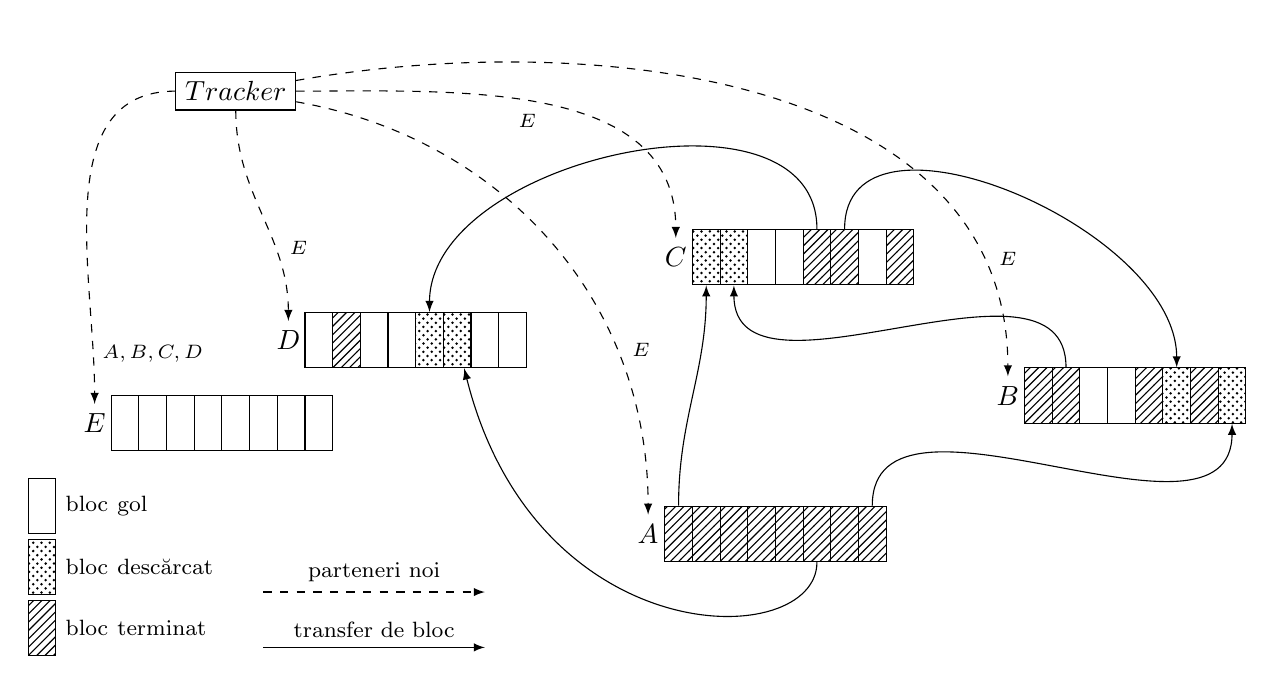
\begin{tikzpicture}[x=10pt, y=10pt]
        \tikzstyle{gol}  = [draw, inner sep=0pt, minimum height=20pt, minimum width=10pt]
        \tikzstyle{des}  = [draw, inner sep=0pt, minimum height=20pt, minimum width=10pt, pattern=crosshatch dots]
        \tikzstyle{cmp}  = [draw, inner sep=0pt, minimum height=20pt, minimum width=10pt, pattern=north east lines]
        \tikzstyle{tran} = [->, >=latex]
        \tikzstyle{part} = [->, >=latex, dashed]

        % Desenează partenerii.
        \foreach \x/\y/\cod/\na/\nb/\nc/\nd/\ne/\nf/\ng/\nh in {
                  2/ 0/A/cmp/cmp/cmp/cmp/cmp/cmp/cmp/cmp,
                 15/ 5/B/cmp/cmp/gol/gol/cmp/des/cmp/des,
                  3/10/C/des/des/gol/gol/cmp/cmp/gol/cmp,
                -11/ 7/D/gol/cmp/gol/gol/des/des/gol/gol,
                -18/ 4/E/gol/gol/gol/gol/gol/gol/gol/gol} {
            \node (\cod) at (\x-0.1,\y) {$\cod$};
            \foreach[count=\c] \n in {\na,\nb,\nc,\nd,\ne,\nf,\ng,\nh}
                \node[\n] (\cod\c) at (\x+\c,\y){};
        }

        % Nodul tracker.
        \node[draw] (tracker) at (-13, 16) {$Tracker$};

        % Liniile de transfer.
        \draw[tran] (A8) edge[out=90, in=-90] (B8);
        \draw[tran] (A1) edge[out=90, in=-90] (C1);
        \draw[tran] (B2) edge[out=90, in=-90] (C2);
        \draw[tran] (C5) edge[out=90, in=90]  (D5);
        \draw[tran] (C6) edge[out=90, in=90]  (B6);
        \draw[tran] (A6) .. controls ([yshift=-1.5cm] A6) and ([xshift=1cm, yshift=-4cm] D6) .. (D6);

        % Liniile de parteneri noi.
        \draw[part] (tracker) edge[out=180, in=90] node[very near end,       right]{\scriptsize{$A, B, C, D$}} (E);
        \draw[part] (tracker) edge[out=-90, in=90] node[     near end, above right]{\scriptsize{$E$}} (D);
        \draw[part] (tracker) edge[out=-10, in=90] node[     near end, above right]{\scriptsize{$E$}} (A);
        \draw[part] (tracker) edge[out=  0, in=90] node[       midway,  below left]{\scriptsize{$E$}} (C);
        \draw[part] (tracker) edge[out= 10, in=90] node[very near end, above right]{\scriptsize{$E$}} (B);

        % Legenda figurii.
        \tikzstyle{textul} = [node distance=1.6cm, inner sep=0pt, anchor=west, text width=2.6cm]
        \draw[part] (-12,-2.1) -- node[above]{\footnotesize{parteneri noi}} (-4,-2.1);
        \draw[tran] (-12,-4.1) -- node[above]{\footnotesize{transfer de bloc}} (-4,-4.1);

        \node[gol] (nodgol) at (-20,1){};
        \node[textul, right of=nodgol]{\footnotesize{bloc gol}};

        \node[des] (noddes) at (-20,-1.2){};
        \node[textul, right of=noddes]{\footnotesize{bloc descărcat}};

        \node[cmp] (nodcmp) at (-20,-3.4){};
        \node[textul, right of=nodcmp]{\footnotesize{bloc terminat}};
    \end{tikzpicture}

    \caption{Exemplu de funcționare a protocolului BitTorrent. Cel care a creat torentul este $A$ și are toate
    blocurile. $E$ este partenerul cel mai recent intrat în roi.}
\end{figure}

Pentru a descărca fișierele din torent un utilizator trebuie să procure fișierul \cod{.torrent} (care este de o
dimensiune mică) și să-l încarce în aplicația sa. Aceasta se conectează la serverele \eng{tracker} și primește lista de
parteneri. Aplicația va comunica cu aceștia pentru a afla ce blocuri au și va putea începe descărcarea în ordinea
dorită, posibil aleatoare. Deoarece și el a fost adăugat la lista de parteneri de către server, alții vor face cerere
la blocurile pe care le are el. Deci pe măsură ce descarcă, va trebui să servească cererile de încărcare spre alții. Cu
cât sunt mai mulți parteneri cu atât crește posibilitatea de a descărca de la mai mulți în același timp și posibilitatea
ca să existe un partener pentru care viteza de transfer să fie mai mare (spre exemplu dacă sunt apropiați geografic, fac
parte din aceeași rețea de mare viteză ș.a.).

Deoarece un \eng{tracker} este necesar doar pentru găsirea de parteneri, traficul generat de server este mic. În plus,
faptul că serverul nu reține pentru niciun moment bucăți din fișiere îl protejează de consecințele legale legate de
posibila încălcare a drepturilor de autor.

La început, pentru găsirea de parteneri, era neapărat nevoie de un \eng{tracker}, dar mai recent se pot găsi parteneri
folosind un tabel distribuit de dispersie. Astfel a devenit posibilă transferarea de fișiere prin BitTorrent fără un
server central.

Totuși găsirea fișierelor \cod{.torrent} nu este descentralizată total. De obicei ele se descarcă de pe servere
\acr{HTTP}. Aici apare și problema dezorganizării. Cu cât un sistem este mai descentralizat cu atât este mai greu să
organizezi fișierele. Torentele nu mai pot fi modificate după creare și sunt identificate în mod unic\footnote{Dar
teoretic pot exista coliziuni.} prin codul \acr{SHA-1}. De asemenea fișierele torent nu pot fi imbricate pentru a forma
structuri ierarhice, deși fișierele conținute sunt organizate. Se întâmplă deseori ca aceleași fișiere să fie încărcate
de mai multe ori sub denumiri puțin diferite sau să fie incluse din nou în torente mai cuprinzătoare. Această duplicare
este defavorabilă deoarece parteneri care ar fi putut comunica sunt astfel separați.

Unele servere \eng{tracker} permit accesul doar utilizatorilor înregistrați. Acestea se numesc servere private și de
obicei necesită o invitație pentru înregistrare. Utilizatorilor le este impusă menținerea unui anumit raport între ce
descarcă și ce încarcă. Pe serverele publice cineva poate chiar să blocheze încărcarea și doar să descarce. Asta
înseamnă că, pe serverele private, viteza de descărcare va fi mai mare pentru că sunt mai mulți parteneri care au
torentul complet și doar încarcă. Problema aici este că fișierele populare vor avea foarte mulți parteneri și cele puțin
populare vor fi chiar uitate. Așa se întâmplă că există fișiere cu ofertă mare și cerere mică și fișiere cu cerere mai
mică, dar fără ofertă.

BitTorrent are și probleme legate de anonimitate. Un \eng{tracker} transmite lista de parteneri fără
criptare.\footnote{Sunt totuși servere \eng{tracker} (ex: opentracker) care adaugă adrese generate aleator pentru ca
adresele \acr{IP} reale să aibă negare plauzibilă.} Deci un agent care intră în roi poate afla adresele \acr{IP} a celor
care descarcă fișiere. Acest lucru poate avea consecințe legale negative pentru cei care fac piraterie, dar și pentru
dizidenții care descarcă și încarcă fișiere nepermise din țările cu regim politic opresiv.

BitTorrent este un protocol cu succes dovedit mai ales de traficul pe care îl generează pe internet.

\subsection{Direct Connect} % ------------------------------------------------------------------------------------------

Direct Connect este un protocol popular \eng{peer-to-peer} inventat în 1999. Protocolul nu are o specificație oficială
și clientul original nu era cu sursă publică\cite{dircon}. Alte programe au fost făcute prin analiza programului
original.

Utilizatorii se conectează la servere (numite \eng{hub}-uri) care rețin lista de fișiere pentru fiecare utilizator și
funcționează ca un intermediar. Comunicarea se realizează printr-un protocol text necodificat. Utilizatorii trimit
căutările la server și acesta întoarce lista de fișiere care se potrivesc de la diferiții utilizatori. 

Pentru descărcarea fișierelor, partenerii comunică între ei. Partajarea de fișiere se bazează pe conceptul de
\eng{slot}. Fiecare utilizator are un număr fix de conexiuni pe care le permite pentru încărcarea de fișiere și altul
pentru descărcare. Acest număr este hotărât de utilizator, dar serverele pot refuza conectarea pe baza asta.

Deoarece utilizatorii comunică des cu serverul, acesta nu admite un număr foarte mare de utilizatori. Problema asta este
rezolvată parțial prin faptul că utilizatorii se pot conecta la mai multe servere simultan.

O altă problemă este faptul că nu există o stare a fișierului (cum este la BitTorrent) care să fie menținută constant pe
internet. Un utilizator alege de la cine vrea să descarce, dar acesta poate pleca. Pentru a continua descărcarea, poate
să caute fișierul după rezumatul \acr{TTH}, dar dacă nu este găsit nu mai poate face nimic decât să aștepte revenirea
posesorului deoarece fișierul nu este păstrat continuu în rețea.

La fel ca BitTorrent, Direct Connect nu protejează identitatea utilizatorilor. Protocoalele care nu criptează
comunicarea pot fi blocate sau încetinite de către \acr{ISP}-uri. Acest lucru s-a întâmplat la BitTorrent\cite{torrblk}.

\subsection{Gnutella} % ------------------------------------------------------------------------------------------------

Gnutella a fost inventat în 2000 și a fost primul protocol \eng{peer-to-peer} total
descentralizat.\cite{gnut1}\cite{gnut2}

Nu există niciun server central sau servere centrale separate (cum sunt la Direct Connect). La deschidere, aplicația se
conectează la parteneri de care află prin diferite metode (liste de utilizatori se află pe internet). Când
utilizatorul vrea să caute ceva, trimite căutarea la toți partenerii cu care este conectat. Aceștia trimit mai departe
căutarea pentru un număr prestabilit de ori (la momentul de fața 4). Răspunsurile la căutări sunt trimise înapoi la cel
ce a inițiat căutarea. Apoi utilizatorul poate să inițieze descărcarea direct de la deținător.

Versiunile recente au modificat structura rețelei pentru a fi mai bine adaptată la numărul mare de parteneri. Acum
sunt două tipuri de noduri: nod frunză, adică utilizator normal care este conectat la un număr mic de parteneri
și nod \eng{ultrapeer} care este conectat la foarte multe noduri \eng{ultrapeer}.

Gnutella are aceeași problemă ca Direct Connect la persistența fișierelor. Fiecare utilizator pune la dispoziție ce
fișiere vrea și când pleacă este posibil ca acestea să nu mai existe în rețea.

În plus, fiind o rețea total descentralizată, conținutul nu este organizat deloc. Pentru Direct Connect \eng{hub}-urile
deseori au un subiect sau reprezintă o anumită zonă geografică, dar pentru Gnutella nu este posibil așa ceva. 

\subsection{Freenet} % -------------------------------------------------------------------------------------------------

Freenet a fost inventat în 2000 și este un \eng{data store}\footnote{Un \eng{data store} este o rețea care reține
informații și le distribuie pentru a fi accesibile și când nodul creator nu este prezent. BitTorrent este un fel de
\eng{data store} la nivel de torent, în sensul că un torent are o stare care e disponibilă cât timp partenerii sunt
conectați, dar fișierele din el nu pot fi modificate. Majoritatea protocoalelor \eng{peer-to-peer} (Direct
Connect, Gnutella ș.a.) nu au \eng{data store}.} distribuit, descentralizat și făcut pentru a fi greu de
cenzurat\cite{freenet}\cite{wikifn}.

Comunicarea în Freenet este criptată și trece prin multe noduri ale rețelei pentru îngreunarea detectării nodului care
trimite, nodului care furnizează și mai ales a informației.

\begin{figure}[t]
    \centering
    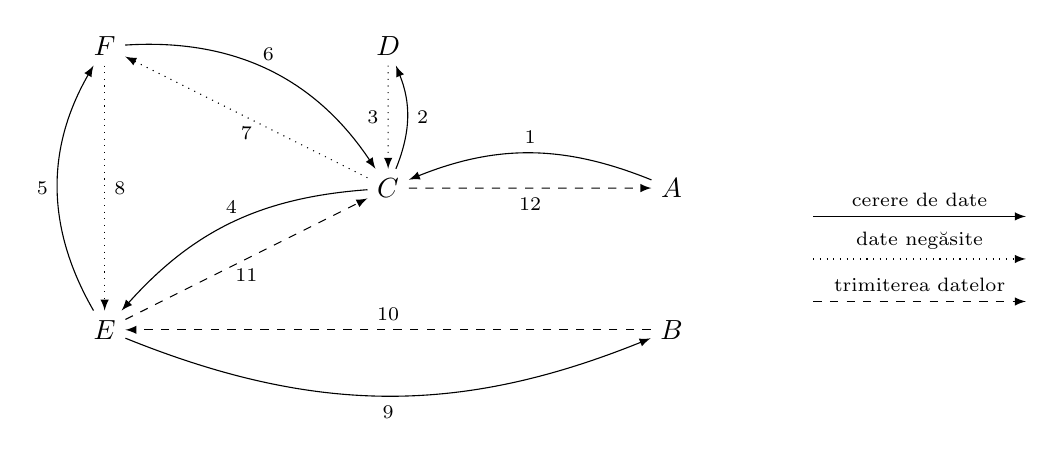
\begin{tikzpicture}[scale=1.8]
        % Desenează punctele.
        \node (D) at (2,2) {$D$};
        \node (F) at (0,2) {$F$};
        \node (C) at (2,1) {$C$};
        \node (A) at (4,1) {$A$};
        \node (E) at (0,0) {$E$};
        \node (B) at (4,0) {$B$};

        % Desenează liniile.
        \tikzstyle{sageata} = [->, >=latex, font=\scriptsize]
        \path[sageata, bend right=22]
            (A) edge node[above]{ 1} (C)
            (C) edge node[right]{ 2} (D)
            (C) edge node[above]{ 4} (E)
            (E) edge node[below]{ 9} (B);
        \path[sageata, bend left]
            (E) edge node[left ]{ 5} (F)
            (F) edge node[above]{ 6} (C);
        \path[sageata, dotted]
            (D) edge node[left ]{ 3} (C)
            (C) edge node[below]{ 7} (F)
            (F) edge node[right]{ 8} (E);
        \path[sageata, dashed]
            (B) edge node[above]{10} (E)
            (E) edge node[below]{11} (C)
            (C) edge node[below]{12} (A);

        % Explică tipul liniilor.
        \path[sageata        ] (5,0.8) edge node[above]{cerere de date    } (6.5,0.8);
        \path[sageata, dotted] (5,0.5) edge node[above]{date negăsite     } (6.5,0.5);
        \path[sageata, dashed] (5,0.2) edge node[above]{trimiterea datelor} (6.5,0.2);
    \end{tikzpicture}

    \caption{Exemplu de comunicare în Freenet. $A$ cere un fișier care se întâmplă să fie reținut de $B$. Numerele
    indică ordinea comunicării.}
\end{figure}

Aplicația Freenet este făcută să ruleze în fundal. Utilizatorul donează o parte din spațiul de pe disc pentru stocarea
de fișiere și aplicația menține starea rețelei prin duplicarea de fișiere și servirea lor la cererea altora. Modul de
interacțiune cu utilizatorul este separat. Freenet furnizează o interfață \acr{HTTP} pentru comunicarea utilizatorului
cu rețeaua. Acesta poate fi accesată din orice navigator \eng{web}.

Fișierele sunt stocate în format criptat, ceea ce înseamnă că este greu chiar și pentru noduri să afle ce fișiere dețin
(pentru a avea negare plauzibilă). Fișierele sunt identificate prin codul \acr{SHA-256} și rețeaua funcționează ca un
tabel distribuit de dispersie.

Freenet este folosit în principal pentru publicarea de \eng{freesites} (pagini \acr{HTML} găsite în rețea). Acestea
conțin legături spre fișiere de interes.

Datorită faptului că fișierele sunt transferate prin mai multe noduri și criptate pe parcurs, viteza de transfer are de
suferit mult.

Problema la un \eng{data store} descentralizat total este că utilizatorii rău intenționați pot adăuga fișiere mari care
n-au niciun rost. Totuși, Freenet este făcut să avantajeze fișierele cerute des. Acestea sunt reținute pe nodurile prin
care trebuie să treacă pentru a ajunge la solicitant și deci încercarea de a afla identitatea celor care rețin un anumit
fișier are ca efect răspândirea mai largă a fișierului.

\section{Sisteme de fișiere distribuite} % =============================================================================

„Un sistem de fișiere distribuit este orice sistem care permite accesul la fișiere pentru mai multe gazde într-o
rețea. Clienții nu au acces la mediul de stocare, ci interacționează printr-un protocol.“\cite{wikidfs}

Astfel de sisteme sunt de obicei concepute pentru a fi folosite într-un \acr{LAN} unde nodurile sunt cunoscute. Din
această cauză multe dintre problemele găsite la sistemele \eng{peer-to-peer} nu există aici.

\subsection{\acr{NFS}} % -----------------------------------------------------------------------------------------------

Network File System (\acr{NFS}) este un sistem de fișiere distribuit conceput în 1984. Prima versiune și modificările
ulterioare sunt descrise în \acr{RFC}-urile 1094\cite{rfc1094}, 1813, 3010, 3530 și 5661.

\acr{NFS} folosește sistemul de apelare de proceduri la distanță numit Open Network Computing \acr{RPC} care este bazat
pe convențiile de apelare folosite în Unix și limbajul C. Datele sunt serializat în formatul External Data
Representation (\acr{XDR}) și trimise prin \acr{UDP} sau \acr{TCP}.

Protocolul inițial este conceput pentru a fi fără stare acolo unde este posibil. Spre exemplu toate procedurile
protocolului erau sincrone. Acest lucru permitea unui client să fie sigur că informațiile (blocuri, metadate și restul)
sunt stocate corect pe partea serverului atunci când procedura se termină. 

Modelul sistemului de fișiere este unul ierarhic care este conceput pentru a fi multiplatformă. Spre exemplu, se caută
câte o singură componentă a căii la un moment dat pentru că nu există un separator de cale comun pentru toate sistemele
de operare.

Operații posibile sunt: crearea, citirea și ștergerea de fișiere și directoare; scrierea în fișiere; crearea de legături
fizice și simbolice; și citirea atributelor sistemului de fișiere.

Datorită faptului că serverul poate fi fără stare, el nu poate ști cu siguranță care fișiere sunt deschise. Prin urmare,
verificarea permisiunilor se face la fiecare operație asupra fișierelor și nu numai la deschidere ca la sistemele de
fișiere locale. În plus, datorită faptului că permisiunile pot fi schimbate în timp ce se modifică fișierul, \acr{NFS}
specifică faptul că autorul unui fișier va avea mereu drepturi depline asupra fișierului indiferent de permisiunile
fișierului.

În versiunea 3 a fost adăugată scrierea asincronă pentru a mări performanța.

În versiunea 4 a fost adăugat și un protocol cu stare și deci operații de deschidere și închidere. Au fost adăugate și
operații compuse. Spre exemplu se poate căuta, deschide și citi un fișier printr-o singură apelare de procedură.

\subsection{\acr{SMB}} % -----------------------------------------------------------------------------------------------

Server Message Block (\acr{SMB}) este un protocol care permite accesul la resurse (imprimante, porturi seriale și
altele) dintr-o rețea de calculatoare, însă cea mai mare parte a lui o constituie accesul la sisteme de fișiere. El a
fost creat inițial la \acr{IBM} fiind modificat ulterior de către Microsoft. Inițial funcționa peste protocolul
\acr{NetBIOS}, dar acum funcționează direct peste \acr{TCP}.

Este optimizat pentru accesul într-o subrețea și, fiind creat de Microsoft, este în mare parte folosit pe calculatoare
cu Windows în rețele \acr{LAN} numite Microsoft Windows Network.

\acr{SMB} este un protocol închis și inițial specificațiile nu erau publicate. Samba este un program cu sursă publică
care permite accesul calculatoarelor ce rulează sisteme de operare de tipul Unix la \acr{SMB}. El a fost construit prin
dezasamblarea protocolului \acr{SMB} folosind inginerie inversă.

\section{Sisteme de fișiere distribuite \eng{peer-to-peer}} % ==========================================================

Există la momentul de față mai multe sisteme de fișiere \eng{peer-to-peer}\cite{wikip2ps}, dar sunt puțin cunoscute și
aproape nefolosite.

\textbf{\acr{CFS}} era un sistem de fișiere ce permitea doar citirea și era bazat pe unul dintre primele tabele
distribuite de dispersie create numit Chord.

\textbf{Infinit} era un sistem de fișiere care promitea multe și a anunțat că va avea o versiune alfa în mai 2010, dar a
fost abandonat cu totul.

\textbf{ColonyFS} pune accent pe anonimitate, securitate și încredere. Se dorește a fi folosită tehnica \acr{FRS}
(\eng{fragmentation redundancy scattering}) pentru împărțirea blocurilor. Și acest proiect a fost abandonat.

\subsection{Ivy} % -----------------------------------------------------------------------------------------------------

Ivy este un sistem de fișiere \eng{peer-to-peer} ce permite citirea, dar și scrierea\cite{lucivy}. Sistemul nu necesită
încrederea tuturor participanților.

El este bazat pe \acr{TDD}-ul numit DHash în care sunt memorate toate datele. Asta înseamnă că modificările fiecărui
utilizator sunt accesibile indiferent de prezența autorului. Cu Ivy, fiecare utilizator are un jurnal care descrie
sistemul de fișiere. Vizualizarea sistemului se realizează prin consultarea tuturor jurnalelor, dar modificarea se
efectuează doar în cel personal. Deci dacă un utilizator este de neîncredere se pot elimina modificările lui foarte
ușor, dar fiecare utilizator decide cine este de încredere și cine nu.

Pentru a mări performanța, Ivy ține minte starea sistemului de fișiere și nu verifică jurnalele la fiecare operație.

Participanții la un sistem de fișiere Ivy nu comunică deloc între ei decât prin DHash. Deoarece comunicare se
realizează exclusiv printr-un \acr{TDD}, acesta poate fi înlocuit cu altul dacă este nevoie.

Ivy se comportă pe sistemul local ca un server de fișiere \acr{NFS}. Deci sistemul de operare trebuie să știe cum să
utilizeze un sistem \acr{NFS} pentru a lucra cu Ivy.

O mare problemă la Ivy este că nu a fost conceput pentru rețele mari cu multe noduri. Pentru un sistem de fișiere care
are mii de noduri sunt foarte multe jurnale de procesat.

Faptul că se folosește un sistem \acr{TDD} înseamnă că oricine poate să scrie cât vrea și nu pot fi impuse limite de
spațiu. Pentru fiecare sistem, spațiu pare nelimitat, dar se adună pe calculatoarele celor care sunt în rețeaua
tabelului distribuit de dispersie.

În plus, nu se poate pune o prioritate pe fișier. Unele fișiere sunt mai căutate decât altele, dar nu există o
autoritate centrală care să decidă multiplicitatea blocurilor.

După măsurătorile făcute de cei care au construit Ivy, sistemul este în medie de 3 ori mai încet decât \acr{NFS}.

\subsection{Pastis} % --------------------------------------------------------------------------------------------------

Pastis este un sistem de fișiere \eng{peer-to-peer} care e creat pentru a putea fi utilizat chiar și pentru sute
de mii de noduri\cite{lucpastis}.

Pastis folosește tabelul distribuit de dispersie numit Past cu implementarea cu sursă publică FreePastry. Deci toate
problemele de la Ivy care sunt cauzate de faptul că se folosește un \acr{TDD} se găsesc și aici.

În Pastis fiecare fișier are un cod \eng{inode} care identifică structura ce memorează datele despre fișier. Această
structură conține lista de blocuri. La fel ca la Ivy, blocurile sunt memorate în \acr{TDD}.

După măsurătorile făcute de cei care au construit Pastis, sistemul este în medie între 1,4 și 1,8 ori mai încet decât
\acr{NFS}.

\section{Tehnologii înrudite} % ========================================================================================

Unele protocoale sunt comune mai multor sisteme de partajare de fișiere. Spre exemplu tabelele distribuite de dispersie
au fost folosite de la început de către Pastis și Ivy, dar a fost adăugat ulterior la BitTorrent ca o metodă de găsire
de parteneri noi.

\acr{TDD}-urile furnizează o metodă de comunicare descentralizată pentru găsirea de valori în funcție de un cod asociat,
astfel simulând un tabel de dispersie.

Pentru un sistem descentralizat, un \acr{TDD} are avantajul că funcționează bine de la câteva sute de noduri până la
milioane de noduri. Ele contactează în medie $\log(n) $ noduri din rețea pentru a găsi informația căutată. În acest sens
sunt mai similare cu arborii binari decât tabelele de dispersie.

\subsection{Kademlia} % ------------------------------------------------------------------------------------------------

Kademlia este tabel distribuit de dispersie conceput în 2002 și este bazat pe o metrică \acr{XOR}.\cite{luckadem} Sunt
folosite chei și coduri de nod pe $b$ biți. În mod normal $b$ este 160, care este și lungimea la \acr{SHA-1}. Distanța
dintre două noduri $n$ și $m$ este $n \oplus m$ interpretat ca un număr întreg. La intrarea în rețea un nod își alege
codul în mod aleator și construiește un număr de $b$ $k$-liste.

O $k$-listă poate conține maxim $k$ triplete de tipul \uplu{adresă \acr{IP}, port \acr{UDP}, cod de nod}. Într-o
$k$-listă notată $i$, $0 \leq i < b$, ar putea fi adăugate nodurile ale căror distanțe față de codul propriu este între
$2^i$ și $2^{i+1}$. Se observă că listele la distanță mică în practică vor reține un singur nod (deoarece numărul de
noduri posibile, $2^b$, este mult mai mare decât nodurile care vor participa în rețea), iar în $k$-lista de distanța cea
mai mare ar putea intra teoretic jumătate din toate nodurile din rețea, dacă $k$ ar fi destul de mare. În mod normal $k$
este 20, iar dacă lista este plină, un nod nou este adăugat doar dacă unul dintre nodurile prezente nu răspunde la un
mesaj \eng{ping}.

\begin{figure}[h]
    \centering
    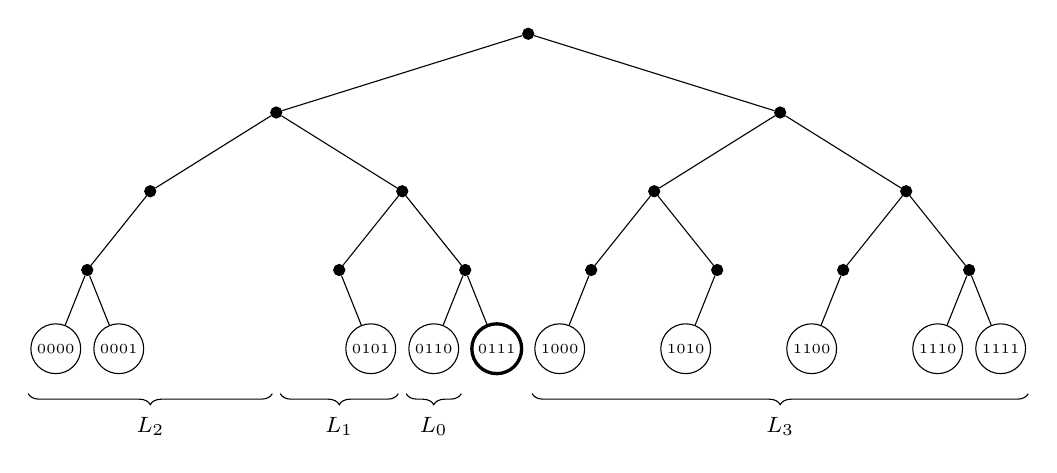
\begin{tikzpicture}[level distance=1.0cm]]
        \tikzstyle{level 1}    = [sibling distance=6.4cm]
        \tikzstyle{level 2}    = [sibling distance=3.2cm]
        \tikzstyle{level 3}    = [sibling distance=1.6cm]
        \tikzstyle{level 4}    = [sibling distance=0.8cm]
        \tikzstyle{every node} = [font=\tiny]
        \tikzstyle{parinte}    = [circle, draw, inner sep=0pt, minimum size=4pt, fill=black]
        \tikzstyle{frunza}     = [circle, draw, inner sep=0pt, minimum size=18pt]

        \node[parinte]{}
            child[sibling angle=10] {node[parinte]{}
                child {node[parinte]{}
                    child {node[parinte]{}
                        child {node[frunza]{0000}}
                        child {node[frunza]{0001}}
                    }
                    child[missing]{}
                }
                child {node[parinte]{}
                    child {node[parinte]{}
                        child[missing]{}
                        child {node[frunza]{0101}}
                    }
                    child {node[parinte]{}
                        child {node[frunza]{0110}}
                        child {node[frunza, very thick]{0111}}
                    }
                }
            }
            child {node[parinte]{}
                child {node[parinte]{}
                    child {node[parinte]{}
                        child {node[frunza]{1000}}
                        child[missing]{}
                    }
                    child {node[parinte]{}
                        child {node[frunza]{1010}}
                        child[missing]{}
                    }
                }
                child {node[parinte]{}
                    child {node[parinte]{}
                        child {node[frunza]{1100}}
                        child[missing]{}
                    }
                    child {node[parinte]{}
                        child {node[frunza]{1110}}
                        child {node[frunza]{1111}}
                    }
                }
            };

        % Desenarea acoladelor.
        \tikzstyle{acoltext} = [midway, yshift=-14pt]
        \tikzstyle{acol} = [decorate, decoration={brace, amplitude=4pt, mirror, raise=2pt}]
        \def\desubt{-4.5}
        \def\marime{0.70}
        \def\La{-1.55}
        \def\Lb{-3.15}
        \def\Lc{-6.35}
        \def\Ld{ 0.05}
        \draw[acol] (\La,\desubt) -- (\La+1*\marime+0.0,\desubt) node[acoltext]{\footnotesize $L_0$};
        \draw[acol] (\Lb,\desubt) -- (\Lb+2*\marime+0.1,\desubt) node[acoltext]{\footnotesize $L_1$};
        \draw[acol] (\Lc,\desubt) -- (\Lc+4*\marime+0.3,\desubt) node[acoltext]{\footnotesize $L_2$};
        \draw[acol] (\Ld,\desubt) -- (\Ld+8*\marime+0.7,\desubt) node[acoltext]{\footnotesize $L_3$};
    \end{tikzpicture}

    \caption{Împărțirea unei rețele pe 4 biți din punctul de vedere al nodului 0111. $L_i$ reprezintă nodurile care
    ar putea intra în $k$-lista $i$.}
\end{figure}

Sarcina reținerii perechii \uplu{cheie, valoare} le revine nodurilor care au codul cel mai apropiat de cheie.

Când un nod vrea să afle valoarea pentru o cheie, se uită în $k$-listele sale pentru $\alpha$ cele mai apropiate noduri
de cheia dată folosind metrica \acr{XOR} și trimite acestora cereri prin \acr{UDP} pentru cheia căutată. De obicei
$\alpha$ este 3 și asta permite căutarea asincronă deoarece nu trebuie așteptat răspunsul la toate cererile pentru a
trece la următoarea iterație. Dacă nodul interogat reține valoarea pentru cheie, atunci o întoarce, altfel întoarce $k$
cele mai apropiate noduri (nu neapărat din aceeași listă). Dacă valoarea nu a fost găsită atunci căutarea continuă cu
$\alpha$ cele mai apropiate noduri întoarse.

Unul dintre avantajele Kademlia este rezistența împotriva unor atacuri \acr{DoS}. Într-o $k$-listă intră un nod nou doar
după ce pică unul existent, deci intrarea mai multor noduri malițioase nu va produce ieșirea celor existente și asta
înseamnă că rețeaua va fi mai rezilientă.

Un alt avantaj este legat de metrica \acr{XOR} folosită. Deoarece este unidirecțională, căutarea de chei va converge
spre aceleași căi indiferent de nodul origine cea ce înseamnă că poate fi implementat un \eng{cache}.

%%%%%%%%%%%%%%%%%%%%%%%%%%%%%%%%%%%%%%%%%%%%%%%%%%%%%%%%%%%%%%%%%%%%%%%%%%%%%%%%%%%%%%%%%%%%%%%%%%%%%%%%%%%%%%%%%%%%%%%%
\chapter{Prezentarea sistemului propriu}

Pentru a rezolva o parte din problemele întâlnite la sistemele de partajare a fișierelor discutate în primul capitol
introduc sistemul propriu numit Negura\footnote{Denumirea face aluzie la \eng{cloud storage}.}, un sistem de fișiere
distribuit de tip \eng{peer-to-peer} care își menține starea (deci este un \eng{data store}).

Datorită măririi vitezelor de internet și a populației conectate la internet nu se mai justifică sistemele total
centralizate care nu profită de resursele de viteză și memorie a utilizatorilor săi. În același timp, soluțiile complet
descentralizate sunt foarte anarhice: dezorganizate, ușor de adăugat falsuri etc.

Sistemul folosit de Negura implică faptul că există o autoritate centrală (care poate fi un server sau mai multe)
care decide ce fișiere sunt adăugate și decide cum vor fi răspândite acestea. Serverul nu reține deloc fișiere, ci se
ocupă cu gestionarea răspândirii blocurilor din care sunt alcătuite fișierele.

Deși există o autoritate centrală, sistemul ar putea funcționa în absența ei. El a fost conceput astfel încât să poată
fi extins prin adăugarea unui tabel distribuit de dispersie prin care partenerii pot comunica pentru menținerea stării
sistemului de fișiere în absența serverului sau în paralel față de acesta.

Modelul meu se bazează pe faptul că în practică într-o rețea de partajare a fișierelor doar un număr mic de participanți
creează conținut. Majoritatea sunt consumatori. Protocolul țintește spre a îmbunătăți acest tip organizat de partajare
de fișiere fără crea un sistem complet centralizat care este mai costisitor, ci prin folosirea resurselor celor care
folosesc sistemul.

Protocolul este conceput astfel încât să nu fie nevoie de un server puternic și acesta să fie ușor de înlocuit dacă este
compromis sau se strică. În plus, pot fi configurate ușor servere oglindă deoarece informația de pe server este în mare
parte statică și serverul nu reține starea clienților.

Sunt folosite două perechi de chei: cele ale administratorului și cele ale serverului. Cu cheia serverului sunt semnate
modificările aduse sistemului de fișiere astfel încât un partener să poată avea încredere în autenticitatea datelor
indiferent de sursă. Cheia serverului este semnată cu cheia administratorului și poate fi înlocuită dacă este
compromisă.

Memorarea sistemului de fișiere se realizează în mod distribuit și redundant pe calculatoarele participanților în rețea.
La crearea serverului se hotărăște mărimea unui bloc și numărul minim de blocuri pe care trebuie să-l rețină fiecare
client.

Pentru adăugarea unui fișier, un client trebuie să-l împartă în blocuri și să trimită metadatele semnate la server.
Adăugarea de fișiere este permisă doar celor care au autorizație de la server. Acest lucru este controlat prin
verificarea semnăturii aplicate pe metadate. Dacă fișierul a fost permis, serverul va aloca blocurile lui unor clienți
care vor trebui să le descarce de la autor (la început) și între ei înșiși (pe parcurs).

Modul de alocare a blocurilor pentru diferiți clienți este la discreția serverului. Se poate implementa o politică prin
care fiecare bloc are aceeași multiplicitate astfel încât fiecare fișier să fie la fel de disponibil sau multiplicitatea
blocurilor poate fi bazată pe popularitate. Această popularitate poate fi decisă prin frecvența citirilor dintr-un
fișier, printr-un sistem de votare al partenerilor sau arbitrar de către server.

Fișierele pot fi descărcate segmentat (ca la BitTorrent) sau secvențial pentru difuzarea în formă de flux
(\eng{streaming}) a fișierelor multimedia. Pentru descărcarea secvențială, programul se comportă ca un server \acr{FTP}
pentru că poate fi montat ușor la sistemul de fișiere în Linux sau ca o unitate în Windows.

\section{Protocolul de comunicare} % ===================================================================================

Sistemul a fost conceput astfel încât serverul să fie fără stare. Asta înseamnă că serverul nu trebuie să rețină starea
clienților (spre exemplu dacă un client și-a actualizat lista de alocare sau nu).

Dacă serverul ar menține starea clienților, în eventualitatea unei erori, această stare trebuie reconstruită și acest
lucru ar mări complexitatea serverelor. În sistemul folosit, serverul reține toate informațiile necesare și clienții fac
cereri. Dacă serverul pică sau clientul întâlnește o eroare înainte să primească răspunsul, clientul nu are decât să
repete cererea.

Comunicare este sincronă se realizează printr-o cerere și un răspuns. Acest lucru simplifică mult complexitatea
serverelor. Faptul că e sincronă înseamnă că un client trebuie să aștepte răspunsul serverului.

Mesajele transmise sunt serializate cu \acr{JSON}. Am ales acest format deoarece este destul de compact și foarte
flexibil față de un format binar și permite mult mai ușor experimentarea și deci e mai ușor de evoluat protocolul.
Pentru mărirea performanței, \acr{JSON} ar putea fi înlocuit într-o versiune ulterioară cu un format binar.

Șirurile de caractere din mesajele \acr{JSON} trebuiesc codate în \acr{UTF-8}.

Toate mesajele de solicitare conțin următoarele câmpuri comune:

\begin{itemize}
\item \cod{request}: denumirea cererii la care trebuie să răspundă;
\item \cod{protocol}: versiunea protocolului folosită de inițiatorul cererii;
\item \cod{software}: denumirea și versiunea aplicației folosite de inițiator.
\end{itemize}

Răspunsurile trebuiesc să fie într-o versiune identică a protocolului sau eventual mai mică dacă este compatibil
răspunsul.

În mod similar, toate răspunsurile vor include câmpurile \cod{protocol} și \cod{software}. În plus, mesajul de răspuns
poate conține un câmp \cod{error} care conține textul unei erori. În acest caz, mesajul nu trebuie să conțină toate
câmpurile specifice acelui tip de răspuns. Spre exemplu, dacă inițiatorul trimite o cerere cu o versiune a protocolului
neînțeleasă de receptor el va trimite un mesaj cu cele două câmpuri obligatorii și câmpul de eroare.

Toate codurile pentru resurse (blocuri, operații și restul) încep de la 1 și cererile pentru ele au ca parametru codul
după care să se întoarcă rezultatele (ele fiind ordonate). Deci un client nou, sau unul care vrea să recupereze datele,
va trimite codul 0 pentru a primi toate resursele.

\section{Structura sistemului de fișiere} % ============================================================================

Structura sistemului de fișiere este reprezentată printr-o listă ordonată de modificări numite operații. Sunt trei
tipuri de operații: adăugarea unui fișier, mutarea unui fișier (sau echivalent redenumirea lui) și ștergerea unui
fișier. Dosarele nu pot fi create, structura lor fiind dedusă din căile fișierelor. 

Spre exemplu dacă este adăugat un fișier în calea \cod{/imagini/jpeg/soare.jpg} vor fi create dosarele \cod{/imagini} și
\cod{/imagini/jpeg} dacă acestea nu existau. La mutarea sau ștergerea fișierelor, dosarele care rămân goale sunt
eliminate. Am ales această metodă de a opera numai pe fișiere deoarece dosarele goale nu au niciun rost și oricum
trebuie specificată calea fișierului în ierarhia de dosare la fiecare operație. În plus se simplifică protocolul.

Limitarea caracterelor posibile în calea unui fișier este aceeași care este des întâlnită la sistemele de fișiere pentru
Unix. Caracterul de separare este bara oblică (\cod{/}). Caracterul nul este interzis din calea unui fișier și denumirea
unui fișier sau dosar nu poate să conțină bară oblică. Dacă sunt mai multe caractere bară oblică succesive, ele vor fi
considerate echivalente cu unul singur. În plus, calea unui fișier nu are limită de lungime și este în Unicode folosind
codarea \acr{UTF-8}.

\section{Rezumat criptografic} % =======================================================================================

Pentru rezumat am ales \acr{SHA-256} pentru fișiere și la fel pentru blocuri. Conform unui test de
performanță\cite{testrez}, acestea sunt vitezele pentru diferiți algoritmi:

\begin{center}
    \begin{tabular}{l r}
        Algoritm      & Viteză    \\
        \hline
        \acr{MD5}     & 255 MiB/s \\
        \acr{SHA-1}   & 153 MiB/s \\
        \acr{SHA-256} & 111 MiB/s \\
        \acr{SHA-512} &  99 MiB/s \\
    \end{tabular}
\end{center}

Dar sunt cunoscute numeroase atacuri pentru \acr{MD5} și \acr{US-CERT} spune că „ar trebui considerat spart din punct de
vedere criptografic și impropriu pentru utilizarea în continuare“\cite{md5broken}, iar \acr{SHA-1} are vulnerabilități
care sunt deocamdată impractice\cite{sha1crypt}.

Pentru sisteme de fișiere cu foarte multe blocuri, memorarea rezumatului pe 256 de biți va crea metadate foarte mari. În
acest caz se poate opta pentru o trunchiere la 192, 160 sau 128 de biți.

\section{Blocuri} % ====================================================================================================

Blocurile reprezintă subdiviziuni de mărime egală a fișierelor. O posibilă excepție este ultimul bloc al unui fișier
care poate avea o mărime mai mică. Mărimea blocurilor trebuie să fie o putere a lui 2 și este decisă la crearea
serverului, ea neputând fi modificată ulterior.

Mărimile de bloc prea mari irosesc spațiu, mai ales dacă sunt memorare fișiere mai mici, dar mărimile prea mici produc
multă meta-informație care trebuie trimisă între server și clienți; și între parteneri. Mărimea recomandată pentru un
bloc este aceeași ca la BitTorrent: între 256~KiB și 1~MiB.

Un bloc este reprezentat printr-un obiect \acr{JSON} cu următoarele câmpuri:

\begin{itemize}
    \item \cod{bid}: codul blocului;
    \item \cod{hash}: rezumatul \acr{SHA-256} pentru bloc (reprezentare hexazecimală);
\end{itemize}

\section{Operații} % ===================================================================================================

Operațiile sunt memorate ca obiecte \acr{JSON} și au următoarele câmpurile comune: 

\begin{itemize}
    \item \cod{oid}: codul crescător al operației pornind de la 1;
    \item \cod{type}: tipul operației;
    \item \cod{date}: data efectuării modificării în formatul stampilă de timp Unix;
    \item \cod{signature}: semnătura aplicată pe această operație în forma șir de caractere în baza~64.
\end{itemize}

Câmpul \cod{type} are valoare \cod{"add"} pentru adăugarea unui fișier, \cod{"move"} pentru mutare și \cod{"delete"}
pentru ștergere.

Semnătura unei operații este calculată peste reprezentarea obiectului \acr{JSON} într-o formă canonică din care este
eliminat câmpul \cod{signature}. Forma canonică se obține în felul următor: toate câmpurile din reprezentare sunt
ordonate alfanumeric și sunt eliminate caracterele albe. Rezultatul este semnat cu cheia privată a serverului.

\subsection{Adăugarea unui fișier} % -----------------------------------------------------------------------------------

Operația de adăugare de fișier are următoarele câmpuri în plus:

\begin{itemize}
    \item \cod{path}: calea fișierului;
    \item \cod{size}: mărimea fișierului în octeți;
    \item \cod{hash}: rezumatul \acr{SHA-256} a fișierului (reprezentare hexazecimală);
    \item \cod{blocks}: lista ordonată de obiecte de tip bloc;
    \item \cod{firstbid}: codul primului bloc;
    \item \cod{lastbid}: codul ultimului bloc.
\end{itemize}

Deoarece codurile pentru blocuri sunt mereu alocate succesiv pentru un fișier, toate blocurile pentru un fișier pot fi
identificate doar prin specificarea primului cod (\cod{firstbid}) și a ultimului (\cod{lastbid}).

Operația de adăugare are două forme: cea completă și cea trunchiată în care nu este prezent câmpul \cod{blocks}. Forma
trunchiată nu conține toată lista de rezumate pentru blocuri și deci are o dimensiune mult mai mică. Ea poate fi
folosită de cei care vor să memoreze sistemul de fișiere într-o formă mai compactă. Lista de rezumate poate fi
descărcată doar atunci când se descarcă fișierul, sau poate fi ignorată dacă utilizatorul are încredere.

\subsection{Mutarea unui fișier} % -------------------------------------------------------------------------------------

Mutarea implică doar schimbarea locației unui fișier, fără a afecta conținutul. Redenumirea este doar mutarea sub un alt
nume. Operația de mutare are următoarele câmpuri în plus:

\begin{itemize}
    \item \cod{path}: calea fișierului care va fi mutat;
    \item \cod{new-path}: noua cale în care va fi pus fișierul.
\end{itemize}

\subsection{Ștergerea unui fișier} % -----------------------------------------------------------------------------------

Ștergerea doar scoate fișierul din ierarhie. Pentru eliminarea completă a fișierului trebuiesc eliminate blocurile din
care este alcătuit. Acest lucru se face separat. Când un fișier este șters, serverul trebuie să modifice listele de
alocare și clienții vor ști că trebuie să elimine blocurile când își actualizează listele.

Operația de ștergere are următoarele câmpuri în plus:

\begin{itemize}
    \item \cod{path}: calea fișierului care va fi șters.
\end{itemize}

\section{Liste de modificare} % ===========================================================================================
\label{sec:limod}

Fiecare partener are un număr de blocuri pe care trebuie să le rețină și pe care trebuie să le încarce la cererea altor
parteneri. Acest număr este decis de către client la intrarea în rețea și este fix. El trebuie să fie între limita
inferioară și superioară decisă de server.

Lista alocată este decisă de către server pentru fiecare client. Ea va varia cu timpul pe măsură ce fișiere sunt
adăugate și șterse, deci se pune problema actualizării ei într-un sistem care trebuie să fie fără stare.

Acest lucru este rezolvat printr-o listă de modificare. Ea este un vector cu indici începând de la 1 și conține numere
pozitive și negative. Numerele pozitive reprezintă codul blocului adăugat și cele negative reprezintă negația codului
șters.

Lista de modificare este ordonată și trebuie văzută ca un ghid asupra ordinii de descărcare a blocurilor. Pe măsură ce
blocurile sunt descărcate trebuie anunțat serverul de completarea lor pentru ca acesta să poată să răspundă la
solicitările clienților pentru partenerii alocați unui bloc.

%%%%%%%%%%%%%%%%%%%%%%%%%%%%%%%%%%%%%%%%%%%%%%%%%%%%%%%%%%%%%%%%%%%%%%%%%%%%%%%%%%%%%%%%%%%%%%%%%%%%%%%%%%%%%%%%%%%%%%%%
\chapter{Funcționarea serverului}

În ceea ce urmează am să descriu cum ar trebui să funcționeze un server și cum ar trebui să răspundă la cererile
clienților.

\section{Crearea serverului} % =========================================================================================

La crearea serverului sunt alese niște date care în mare parte nu mai pot fi modificate mai târziu. Trebuiesc alese
următoarele:

\begin{itemize}
    \item numele serverului, care are scop pur descriptiv;
    \item mărimea blocurilor, care este o putere a lui 2 preferabil între 256~KiB și 1~MiB;
    \item numărul minim de blocuri pe care trebuie să-l rețină un client care vrea să intre în rețea;
    \item numărul maxim de blocuri (pentru cazul în care serverul folosește modelul unui disc virtual prealocat cum am
    implementat eu);
    \item portul pe care se va deschide serverul;
    \item valoarea \cod{check-in-time};
    \item și perechea de chei a administratorului și cea a serverului;
\end{itemize}

După cum am spus și în capitolul precedent, cheia serverului poate fi modificată, dar cheia administratorului este
permanentă. Cheia serverului trebuie stocată pe serverul în funcțiune pentru a permite semnarea operațiilor fără o
prezență umană. Acest lucru înseamnă că există o șansă mai mare ca această cheie să fie compromisă. Dacă acest lucru se
întâmplă, va trebui înlocuită perechea de chei a serverului și eventual șterse operațiile incorecte care au fost
adăugate.

Valoarea \cod{check-in-time} este folosită pentru a informa clienții despre câte secunde ar fi preferabil să aștepte
între solicitări. Un număr mic reduce latența, iar un număr mai mare reduce încărcarea serverului. Serverul ar putea să
blocheze temporar un client dacă acesta nu respectă acest interval.

\section{Informații despre server} % ===================================================================================

Pentru a intra în rețea, un utilizator trebuie să știe informații despre server. Pentru aceasta există cererea
\cod{server-info} care nu are niciun parametru. Aceasta este singura cerere la care un client neînregistrat sigur va
primi un răspuns.

Serverul va răspunde la solicitări cu un mesaj care conține următoarele câmpuri:

\begin{itemize}
    \item \cod{name}: denumirea serverului;
    \item \cod{public-key}: cheia publică a serverului;
    \item \cod{admin-public-key}: cheia publică a administratorului;
    \item \cod{block-size}: mărimea blocurilor folosită de acest server;
    \item \cod{minimum-blocks}: numărul minim de blocuri;
    \item \cod{maximum-blocks}: numărul maxim de blocuri;
    \item \cod{check-in-time}: numărul de secunde de așteptare între solicitări.
\end{itemize}

\section{Înregistrarea} % ==============================================================================================

Pentru ca serverul să răspundă la alte cereri, utilizatorul trebuie să se înscrie pentru a fi luat în evidență. Pentru
asta este cererea \cod{registration} și conține următoarele câmpuri:

\begin{itemize}
    \item \cod{public-key}: cheia publică a clientului;
    \item \cod{number-of-blocks}: numărul de blocuri pe care se oferă clientul să le rețină;
    \item \cod{port}: portul la care clientul va răspunde la cereri;
    \item \cod{permission-code}: un cod de 128 de biți în forma hexazecimală (opțional).
\end{itemize}

Câmpul \cod{permission-code} este opțional și trebuie trimis doar dacă înscrierea se bazează pe invitații.

Serverul va înregistra clientul cu portul specificat și adresa \acr{IP} de la care s-a făcut cererea și va trimite un
răspuns care conține câmpurile:

\begin{itemize}
    \item \cod{registration}: conține \cod{"accepted"} dacă înregistrarea a fost permisă sau \cod{"failed"} altfel;
    \item \cod{uid}: codul care i-a fost dat clientului;
    \item \cod{failed-reason}: mesaj care conține motivul respingerii (opțional).
\end{itemize}

Dacă înregistrarea a eșuat atunci va fi inclus câmpul \cod{"failed-reason"} în care este inclus motivul.

\section{Preluarea blocurilor alocate} % ===============================================================================

După ce a intrat în rețea, un client trebuie să afle lista de blocuri pe care trebuie să le descarce. Pentru asta există
cererea \cod{get-block-list} care întoarce lista de modificări după un anumit index. Această cerere conține următoarele
câmpurile:

\begin{itemize}
    \item \cod{uid}: codul clientului pentru care se cere lista;
    \item \cod{after}: indicele după care să fie întoarsă lista de modificări.
\end{itemize}

Se observă că un client poate accesa și lista altui client, acestea fiind publice.

Serverul răspunde cu un singur câmp \cod{blocks} care conține vectorul de numere ce reprezintă lista de modificări.
Vectorul va fi gol dacă nu s-a făcut nicio modificare între timp.

\section{Verificarea stării sistemului de fișiere} % ===================================================================

Când clientul vrea să verifice dacă s-a actualizat starea sistemului de fișiere trimite cererea \cod{filesystem-state}.
Această cerere conține doar parametrul \cod{after} care specifică codul ultimei operații de care știe clientul și
serverul trebuie să răspundă cu toate operațiile care au fost efectuate după aceasta. Deoarece codul primei operații va
fi mereu 1, clientul trebuie să trimită 0 pentru a primi toate modificările de la început.

Răspunsul va conține un singur câmp, \cod{operations}, care este un vector de operații care au fost descrise în
secțiunea precedentă. Vectorul poate fi gol dacă nu s-a făcut nicio modificare între timp.

\section{Preluarea partenerilor pentru blocuri} % ======================================================================

Pentru descărcarea unor blocuri (pentru că i-au fost alocate sau pentru că dorește fișierele) un client trebuie să afle
ce parteneri dețin acele blocuri. Pentru asta va fi trimisă cererea \cod{peers-for-blocks}. Aceasta are câmpul
\cod{blocks} ce conține lista de coduri de blocuri pentru care se doresc partenerii.

Răspunsul serverului va conține câmpul \cod{blocks} care este un obiect \acr{JSON}. Fiecare câmp reprezintă codul unui
bloc, iar valoarea asociată va fi lista de adrese a partenerilor care au blocul. O adresă este specificată ca un șir de
caractere ce reprezintă o adresă \acr{IP} cu port (exemplu: \cod{"127.0.0.1:5000"}).

După cum este detaliat în secțiunea~\ref{sec:adop}, când un client adaugă un fișier, toate blocurile sunt trecute într-o
listă de blocuri alocate temporar acelui client deoarece el este singurul care le poate încărca celorlalți. Deci lista
de adrese va trebui să conțină și adresa autorului până când expiră alocarea temporară.

\section{Anunțarea blocurilor complete} % ==============================================================================

Din când în când clientul trebuie să anunțe serverul asupra stării listei de blocuri alocate. Pentru aceasta trimite 
mesajul \cod{have-blocks} cu următoarele câmpuri:

\begin{itemize}
    \item \cod{uid}: codul clientului;
    \item \cod{blocks}: lista de blocuri care au fost descărcate.
\end{itemize}

Serverul nu are niciun răspuns pentru această cerere deci va trimite un obiect \acr{JSON} gol.

\section{Adăugarea operațiilor} % ======================================================================================
\label{sec:adop}

Cele trei tipuri de operații nu sunt create de server, ci doar sunt aprobate de acesta. Pentru procesarea unei operații
există cererea \cod{add-operations}. Ea poate fi trimisă de oricine, dar serverul verifică dacă provine de la un
utilizator autorizat prin verificarea semnăturii.

La prima vedere, se pare că serverul ar trebui să respingă cereri care provin de la adrese neautorizate, dar nu este o
idee bună. Un utilizator, folosind cheia corectă, poate opta să adauge operații de la o adresă străină sau un calculator
străin pentru a se separa de contul de utilizator normal.

Într-o singură cerere pot fi adăugate mai multe tipuri de operații. Operațiile de tipul mutare sau ștergere nu necesită
nimic în plus, dar pentru cea de adăugare de fișier trebuiesc mai întâi create blocurile. Ele vor fi stocate într-un
dosar special și fișierul poate fi eliminat.

Această cerere are doar câmpul \cod{operations} care va conține o listă de obiecte de tip operație. Operațiile sunt
incomplete deoarece unele câmpuri pot fi adăugate doar de server. Prin urmare, câmpurile \cod{oid}, \cod{date},
\cod{firstbid}, \cod{lastbid} și toate câmpurile \cod{bid} din \cod{blocks} vor conține valoarea 0. Câmpul
\cod{signature} va conține semnătura clientului.

Serverul va verifica autenticitatea operațiilor și va modifica câmpurile necesare. Pentru fiecare operație, în \cod{oid}
va pune codul primei valori disponibile, în \cod{date} va pune timpul curent și dacă operația este de adăugare de
fișier, va completa codurile de bloc. Operațiile rezultate vor fi semnate cu cheia serverului și vor fi adăugate la
lista de operații.

Blocurile conținute vor fi alocate clienților după un anumit algoritm. Cel folosit în implementarea mea este descris în
secțiunea~\ref{sec:algaloc} de la pagina \pageref{sec:algaloc}. În plus, toate blocurile vor fi trecute în lista de
blocuri temporare pentru autor. În mod normal, blocurile vor fi alocate temporar pentru 24 de ore, după care autorul
poate să le șteargă și serverul nu va mai răspunde cererii \cod{peers-for-blocks} cu adresa lui.

Mesajul de răspuns al serverului va avea câmpul \cod{first-block-ids} care va conține un număr pentru fiecare operație
adăugată în ordine. Numărul va fi codul primului bloc dacă este operație de adăugare de fișier sau 0 altfel. Din acest
câmp se poate deduce codul fiecărui bloc. Autorul are nevoie să știe codurile imediat pentru a răspunde cererilor de
încărcare.

\section{Preluarea rezumatelor} % ======================================================================================

Dacă lista de operații a fost preluată în formă trunchiată, atunci este nevoie să fie luate rezumatele pentru blocuri
dacă se dorește verificarea lor. Pentru acest caz există cererea \cod{hashes-for-blocks}. Unicul parametru este
\cod{blocks} care este o listă de coduri de bloc și răspunsul va conține câmpul \cod{hashes} care este un obiect
\acr{JSON}. Câmpurile obiectului reprezintă codul unui bloc, iar valoarea asociată va fi un șir de caractere ce
reprezintă rezumatul în forma hexazecimală.

%%%%%%%%%%%%%%%%%%%%%%%%%%%%%%%%%%%%%%%%%%%%%%%%%%%%%%%%%%%%%%%%%%%%%%%%%%%%%%%%%%%%%%%%%%%%%%%%%%%%%%%%%%%%%%%%%%%%%%%%
\chapter{Funcționarea clientului}

În ceea ce urmează am să descriu cum ar trebui să funcționeze aplicația client.

Aplicația clientului este menită a funcționa ca un program de fundal majoritatea timpului și este preferabil ca ea să
fie pornită odată cu sistemul pentru a fi cât mai mult timp conectată la rețea.

Aplicația trebuie să aibă opțiuni de limitare a resurselor folosite. Dacă ea nu are opțiuni de limitare și consumă prea
mult trafic când utilizatorul folosește internetul sau prea multe cicluri \acr{UCP} când utilizatorul rulează un joc
intensiv, el va fi nevoit să închidă aplicația. Deci este în interesul autorului să furnizeze opțiuni de limitare.

Sunt două obligații principale pe care le are aplicația: încărcarea blocurilor care i-au fost alocate clientului la
cererea altor parteneri și furnizarea serverului \acr{FTP} către utilizator pentru ca acesta să poată accesa sistemul de
fișiere.

Deci după intrarea unui client în rețea, acesta trebuie să afle lista de blocuri alocate lui, să le descarce în fundal
și să notifice serverul despre terminarea lor. Când un partener face o cerere pentru un bloc terminat, acesta trebuie
să-l încarce, ținând cont de limita de conexiuni simultane și de limita de trafic specificată de utilizator.

\section{Preluarea unui bloc} % ========================================================================================

Pentru a descărca un bloc se folosește un mesaj special. Cererea conține tot un obiect \acr{JSON}, dar răspunsul este un
șir de biți. Obiectul are următoarele câmpuri:

\begin{itemize}
    \item \cod{block-id}: codul blocului care este cerut;
    \item \cod{offset}: decalajul de la care se vor întoarce octeții din bloc (opțional);
    \item \cod{length}: câți octeți vor fi întorși (opțional).
\end{itemize}

Câmpul \cod{offset} este opțional. Dacă el nu este prezent se presupune implicit a fi 0. Câmpul \cod{length} este tot
opțional și va fi implicit mărimea blocului.

Partenerul receptor va răspunde prin a trimite un întreg pe 4 octeți în format \eng{big-endian} care are următoarele
semnificații:

\begin{itemize}
    \item \cod{BLOCK\_FOUND} (valoarea 1): blocul există și urmează a fi trimis;
    \item \cod{BLOCK\_BUSY} (valoarea 2): blocul există, dar partenerul receptor este prea ocupat;
    \item \cod{BLOCK\_NOT\_FOUND} (valoarea 3): blocul nu este prezent la partenerul receptor (posibil din cauză că nu a
    apucat să-l descarce sau partenerul inițiator este dezinformat);
    \item \cod{BLOCK\_INVALID\_LENGTH} (valoarea 4): partenerul inițiator a trimis o lungime invalidă pentru bloc.
\end{itemize}

Dacă este citită valoarea \cod{BLOCK\_FOUND} atunci se va scrie un alt întreg pe 4 octeți care are semnificația de
numărul de octeți care vor fi trimiși. Această valoare este importantă pentru cazul în care partenerul inițiator nu a
inclus câmpul \cod{length}.

Apoi vor fi scriși toți octeții necesari și conexiunea va fi închisă.

În situația în care unui client i-au fost alocate blocuri dintre cele pe care le-a adăugat el (deloc improbabil) atunci
el nu va trebui să le descarce, ci doar le va muta.

\section{Vizualizarea sistemului de fișiere} % =========================================================================

Utilizatorul uman interacționează cu sistemul de fișiere prin serverul \acr{FTP}. Am ales această metodă pentru că multe
sisteme de operare au ca o funcționalitate inclusă interacționarea cu un server \acr{FTP}. În plus, și pentru Windows și
pentru Linux există aplicații care montează servere \acr{FTP} la sistemul de fișiere. Acest lucru înseamnă că un
utilizator poate să folosească fișierele ca și cum ar fi pe sistemul său: poate să încarce un film și să sară la
mijlocul acestuia, poate să încarce un dosar întreg cu fișiere audio în redatorul preferat ș.a.m.d.

Un aspect de notat este că aplicația nu are nevoie să facă \eng{caching} de blocuri deoarece programul de montare a
sistemului \acr{FTP} va face asta oricum. În schimb, aplicația poate descărca anticipat blocuri dintr-un fișier, sau
pentru fișierele dintr-un dosar dacă are motive să creadă că acestea vor fi necesare în viitorul apropriat. Acest lucru
este valabil la difuzarea în flux a fișierelor.

%%%%%%%%%%%%%%%%%%%%%%%%%%%%%%%%%%%%%%%%%%%%%%%%%%%%%%%%%%%%%%%%%%%%%%%%%%%%%%%%%%%%%%%%%%%%%%%%%%%%%%%%%%%%%%%%%%%%%%%%
\chapter{Implementarea sistemului}

În acest capitol discut implementarea propriu-zisă a proiectului. Pentru scriere m-am folosit de GitHub și deci toate
sursele (și implicit versiunile intermediare) sunt disponibile la pagina: \url{https://github.com/paul-nechifor/Negura}

\section{Aspecte} % ====================================================================================================

Sistemul a fost împărțit în trei proiecte: NeguraClient (aplicația client), NeguraServer (aplicația server) și
NeguraCommon (părțile comune aplicațiilor). Proiectele sunt scrise în limbajul Java și au ca rezultat final două fișiere
\acr{JAR} (cele două aplicații) care conțin toate resursele necesare pentru rulare.

\subsection{Proiecte folosite} % ---------------------------------------------------------------------------------------

Am ales limbajul Java, special pentru că este ușor să fie scrise aplicații multiplatformă cu el. Dar biblioteca de
interfață grafică primară (Swing) este nesatisfăcătoare. Deși poate imita interfața grafică nativă cel puțin la
înfățișarea ferestrelor și componentelor, ea nu permite unele aspecte precum utilizarea de meniuri native în zona de
notificare. Din acest motiv am ales biblioteca \acr{SWT} care folosește componentele native ale sistemelor admise.

Deoarece lucrul cu dispunerea componentelor în \acr{SWT} este prea stufoasă, am ales să folosesc biblioteca MigLayout.
Acest gestionar de dispunere folosește comenzi text succinte care pot realiza dispuneri complexe. Modul de lucru poate
fi comparat cu \acr{CSS}.

Pe partea de server trebuie gestionat un număr mare de date, deci a trebuit să folosesc o bază de date. Am ales
PostgreSQL și prin urmare am folosit pachetul care furnizează \eng{driver}-ul \acr{JDBC} pentru lucru cu această bază de
date.  Deoarece serverul folosește intensiv baza de date a trebuit să folosesc un \eng{connection pool}. Am ales Commons
\acr{DBCP}.

Am mai folosit și următoarele biblioteci:

\begin{itemize}
    \item Apache FtpServer pentru crearea serverului \acr{FTP};
    \item Google Gson pentru comunicarea \acr{JSON};
    \item și Commons \acr{CLI} pentru procesarea opțiunilor din linia de comandă.
\end{itemize}

\subsection{Platforme compatibile} % -----------------------------------------------------------------------------------

Scrierea unei aplicații multiplatformă a fost printre primele mele obiective.

Deoarece \acr{SWT} folosește componentele native ale sistemelor admise, el vine în pachete distincte pentru fiecare
sistem. Deci pentru fiecare dintre cele două aplicații și fiecare din sistemele admise trebuie să construiesc pachete
\acr{JAR}. Deși \acr{SWT} este compatibil cu mai multe platforme, eu construiesc aplicațiile doar pentru cele din
tabelul de mai jos pentru că sunt singurele pe care pot să testez.

\begin{center}
    \begin{tabular}{l l r}
        Proiect      & Platformă  & Mărime \acr{JAR} \\
        \hline
        NeguraClient & Linux 32   &         2,908~MB \\
        NeguraClient & Linux 64   &         3,068~MB \\
        NeguraClient & Windows 32 &         3,257~MB \\
        NeguraClient & Windows 64 &         3,244~MB \\
        NeguraServer & Linux 32   &         2,769~MB \\
        NeguraServer & Linux 64   &         2,929~MB \\
        NeguraServer & Windows 32 &         3,118~MB \\
        NeguraServer & Windows 64 &         3,105~MB \\
    \end{tabular}
\end{center}

Am încercat să respect standardele specifice platformei. Spre exemplu, pentru Linux, conform XDG Base Directory
Specification\footnote{\url{http://standards.freedesktop.org/basedir-spec/basedir-spec-latest.html}} dosarul în care se
memorează dosarul de configurare ar trebui să fie \cod{\$XDG\_CONFIG\_HOME} dacă există această variabilă sau
\cod{\$HOME/.config} altfel. Acest lucru nu este respectat de multe aplicații care în schimb poluează dosarul
utilizatorului cu fișiere de configurare. Pe de altă parte, pe sistemul Windows, trebuie utilizat dosarul din variabila
\cod{\%APPDATA\%}.

Un alt aspect pe care-l consider important este internaționalizarea. Cele două aplicații nu au textele din interfața
grafică programate fix în sursă. Ele sunt încărcate automat de către Java dintr-un pachet de resurse (clasa
\cod{ResourceBundle}) în funcție de setările de localizare ale utilizatorului. Aplicațiile nu au opțiuni de schimbare a
limbii (spre diferență de multe aplicații, care după părerea mea procedează incorect), ci ele sunt încărcate automat cu
limba sistemului. 

Limbile existente sunt doar limba română și limba engleză.

\subsection{Alte aspecte comune aplicațiilor} % ------------------------------------------------------------------------

La deschiderea aplicațiilor, acestea caută existența fișierului de setări în dosarul standard de configurare specific
sistemului de operare. Dacă el nu este găsit, atunci aplicația server deschide fereastra de creare a fișierului de
configurație și aplicația client deschide fereastra de conectare la un server.

Fișierele de configurație conțin un obiect serializat în \acr{JSON} cu toate setările. Ele ar putea fi modificate chiar
cu un editor de text.

Ambele aplicații trebuie să deschidă un soclu de server pentru a răspunde la cereri. Pentru performanță am folosit
mulțimea de fire din clasa \cod{ThreadPoolExecutor}. Setările pot fi alterate de către utilizator.

La client și la server, cheile sunt memorate în formă criptată. Pe parola aleasă de utilizator este aplicată funcția de
rezumare \acr{SHA-256} de $n$ ori succesiv. Ultimul rezultat este trunchiat la 128 de biți și aceasta este cheia cu care
se criptează și decriptează perechea de chei folosind \acr{AES-128}. Folosesc \acr{AES-128} pentru că \acr{AES-256} nu
este permis de toate sistemele. Compunerea funcțiilor de rezumare este folosită pentru că îngreunează atacurile de
dicționar. Valoarea pe care o folosesc pentru $n$ este 4000.

Pentru trimiterea mesajelor din istoric folosesc clasa \cod{Logger} cu \cod{FileHandler} pentru memorarea pe disc.

Aplicația server are două interfețe: una grafică (dacă este deschisă fără niciun parametru) și una text (dacă este
deschisă cu opțiunea \cod{-cli}). În lumea Unix este normal ca un program server să fie deschis fără interfață grafică.
Acest lucru permite, spre exemplu, utilizarea aplicației pe un calculator care nu are monitor.  Interfața grafică
permite o serie de vizualizări precum afișarea multiplicităților pentru blocuri și listarea operațiilor din sistem.

La deschidere, aplicația client creează în zona de notificare o iconiță care este interfața principală de lucru. Prin
apăsarea ei se deschide meniul din care se pot selecta acțiuni precum: deschiderea ferestrei de statistici, forțarea
actualizării sistemului de fișiere, deschiderea sau închiderea serverului \acr{FTP} și deschiderea ferestrei de adăugare
de fișiere.

\section{Algoritmul de alocare} % ======================================================================================
\label{sec:algaloc}

Există mai multe modalități de a gestiona distribuirea blocurilor. Eu am ales o metodă bazată pe un disc virtual
prealocat.

La crearea serverului, trebuie ales numărul de blocuri din care va fi compus discul virtual. Numerele blocurilor încep
de la 1 și sunt consecutive. Indiferent dacă un bloc aparține sau nu unui fișier, el poate fi alocat unui client.
Numărul de clienți la care este alocat un bloc se numește multiplicitatea lui. Cu algoritmul acesta se țintește spre a
conferi fiecărui bloc aceeași multiplicitate.

La intrarea unui client în rețea, acesta specifică cele $n$ blocuri pe care se oferă să le rețină. Printr-o singură
comandă \acr{SQL} se selectează $n$ blocuri aleatoare dintre cele cu multiplicitatea cea mai mică. Aceste blocuri îi vor
fi alocate lui, astfel menținându-se multiplicitatea egală. Însă doar cele care aparțin unor fișiere vor fi trecute în
lista lui de alocare.

La asta se referă prealocarea: încă de la înregistrare se știe care sunt cele $n$ blocuri pentru fiecare client, deci nu
va fi nevoie să se calculeze alocarea la fiecare adăugare de fișier.

La adăugarea unui fișier se folosesc mereu primele blocuri libere din stânga. Evident, trebuie să se verifice că sunt
destule, altfel se întoarce o eroare. Deoarece acele blocuri au fost deja alocate, doar se face actualizarea în listele
de alocare.

La ștergerea unui fișier, cele $m$ blocuri ale lui sunt eliminate și se șterg asocierile dintre clienți și acele
blocuri. Asta înseamnă că șirul de blocuri ale discului virtual nu va mai fi continuu și scade dimensiunea lui. După cum
am spus în secțiunea~\ref{sec:limod}, clientul este anunțat despre ștergerea blocurilor prin lista de modificare.
Dimensiunea este readusă la echilibru prin adăugarea a $m$ blocuri noi în dreapta. Fac acest lucru pentru că nu este o
idee bună refolosirea codurilor șterse. Se observă că nu este nevoie să se genereze o nouă alocare pentru blocurile
adăugate. Fiecărui bloc șters îi corespunde unul adăugat, deci se reface asocierea dintre clienți și blocuri pe noile
coduri. 

Această metodă de alocare necesită două operații în plus: expandarea discului virtual și contractarea lui. La o
expandare cu $p$ blocuri, se adaugă $p$ blocuri noi în dreapta. La această operație o să scadă multiplicitatea la toate
blocurile. Fie $v$ numărul de blocuri ale discului virtual și $s$ suma blocurilor stocate de toți clienții.
Multiplicitatea medie este $\frac{s}{v}$. După expandare ea trebuie să fie $\frac{s}{v+p}$. Deci pentru fiecare client
se aleg aleator $\frac{p}{v+p}$ din blocurile sale alocate și se realocă în blocurile noi. Fiecare dintre aceste
realocări se face folosind regula de mai sus pentru a se ajunge la o multiplicitate uniformă.

La contractarea discului virtual cu $p$ blocuri se șterg $p$ blocuri din dreapta. Doar blocurile libere pot fi șterse la
o contractare. Pentru fiecare bloc eliminat, și pentru fiecare client care are acel bloc alocat, se face conexiunea
aleatorie cu unul dintre blocurile rămase folosind regula de mai sus pentru o multiplicitate uniformă.  De data aceasta
se observă că blocurile șterse pot fi refolosite la o viitoare expandare pentru că ele nu au fost niciodată folosite
pentru fișiere.

\section{Studiu de caz} % ==============================================================================================

Am să prezint un mod în care poate fi folosit sistemul implementat de mine într-un caz real.

Cele mai multe dintre distribuțiile Linux nu sunt sponsorizate de către companii și trebuie să se bazeze pe donațiile
utilizatorilor pentru găzduirea serverelor și oglinzilor. Spre exemplu Arch Linux publică un număr mare de pachete care
sunt folosite pentru actualizarea sistemului de operare. Cu timpul, pachetele sunt oglindite pe alte servere. Când un
pachet este actualizat, precedentul este șters. În scurt timp oglinzile fac același lucru.

Protocolului meu poate fi o alternativă pentru distribuirea pachetelor de actualizare de la un număr mic de participanți
(creatorii distribuției) la un număr mare de participanți în rețea (utilizatorii distribuției).

În acest caz nu se dorește criptarea datelor deoarece informația este publică. În plus, datorită faptului că unii
participanți vor dona mai multe resurse decât vor folosi, ar putea fi implementat un server care răspunde și la cererile
clienților neînregistrați, cât timp acest lucru nu afectează în mod negativ sistemul prea mult.

Primul avantaj este că se descongestionează serverul de actualizări. Alt avantaj este că nu va mai fi nevoie să se
șteargă așa de repede pachetele vechi deoarece spațiul disponibil va fi mult mai mare. Unii utilizatori doresc să
instaleze versiuni mai vechi ale programelor pentru că sunt mai stabile, dar în modul de funcționare curent, acestea nu
mai sunt disponibile de pe serverul principal și majoritatea oglinzilor.

%%%%%%%%%%%%%%%%%%%%%%%%%%%%%%%%%%%%%%%%%%%%%%%%%%%%%%%%%%%%%%%%%%%%%%%%%%%%%%%%%%%%%%%%%%%%%%%%%%%%%%%%%%%%%%%%%%%%%%%%
\chapter{Extinderea protocolului}

La proiectarea protocolului a trebuit să țin cont de posibilitatea de al implementa. Nu am vrut să descriu un protocol
sofisticat care ar merge pe hârtie, dar ar fi prea ambițios pentru al putea implementa și a-i testa funcționalitatea.
Dar pe parcurs m-am gândit la niște modificări și adăugiri care îi pot fi aduse.

\section{Accelerarea răspândirii blocurilor} % =========================================================================

Perioada critică în descărcarea unui bloc este imediat după ce el a fost creat. Atunci el există doar pe calculatorul
autorului și toți partenerii care au nevoie de acel bloc (pentru că l-a fost alocat sau doresc fișierul) îl vor solicita
de la un singur client. Ambuteiajul rezultat încetinește răspândirea blocurilor.

O soluție ar fi ca autorul operației să transmită blocurile pe un canal extern la un număr de parteneri înainte de
adăugarea ei. Apoi trimite la server cererea care conține și identitatea acelor parteneri, iar serverul îi va adăuga pe
toți acești parteneri ca având blocuri temporare.

\section{Oglindirea serverului central} % ==============================================================================

O problemă a \acr{TDD}-urilor este forma limitată a comunicării posibile. Tot ce se poate face este căutarea unei valori
în funcție de cheie.

Se pune problema cum poate o mulțime de oameni să facă un sistem de fișiere comun fără a achiziționa servere dedicate
(care sunt scumpe) și cum poate fi protejat acesta. Se caută o soluție mai \emph{ad hoc} care nu necesită o investiție
monetară.  Se presupune că utilizatorii sunt mai reticenți să doneze bani pentru a cumpăra un server, dar au mai puțină
reținere în a dona resursele de spațiu și trafic ale calculatoarelor proprii având în vedere că pot renunța oricând.

Soluția propusa este folosirea unor intermediari voluntari. Liderul creează serverul pe calculatorul său obișnuit și
acesta comunică (posibil criptat) doar cu utilizatorii care doresc a fi oglinzi. Oglinzile au rolul de a răspunde
solicitărilor venite de la clienți și nu pot falsifica operațiile sistemului de fișiere pentru că ele sunt semnate.

\section{Anunțuri de la server} % ======================================================================================

La BitTorrent și alte protocoale, serverul are doar rolul de a răspunde la cereri. Asta creează o problemă când mai
mulți utilizatori așteaptă publicarea un fișier. Ei vor face cereri periodice așteptând apariția fișierului. Drept
urmare, serverul va fi suprasolicitat și utilizatorii vor primi fișierul cu întârziere.

La BitTorrent există o soluție externă protocolului: înscrierea la un flux \acr{RSS}. Dar aceasta nu este standardizată
și tot este bazată pe verificări periodice.

Acest tip de problemă poate fi rezolvată simplu prin implementarea șablonul de proiectare Observator. Ideea este că
utilizatorii înregistrați se pot înscrie să primească notificări când s-a făcut o modificare într-un subdosar. Se pot
crea reguli mult mai sofisticate pentru anunțuri, dar dacă ierarhia sistemului de fișiere este organizată bine, această
regulă de una singură poate fi foarte puternică.

Însă notificările nu sunt obligatorii. Doar pentru că un client nu a fost anunțat de adăugarea unui fișier, nu înseamnă
că nu a fost adăugat. Astfel de cazuri se pot întâmpla când serverul este prea încărcat. În orice caz, aplicația
clientului va depista modificarea subdosarului când face actualizarea listei de operații.

Un alt tip de anunț pe care-l poate primi un client este cel de modificare a listei lui de blocuri. Dacă serverul
optează să trimită aceasta notificare, poate scurta timpul până când fișierele vor fi disponibile spre încărcare cu
viteză maximă.

\section{Simplificarea protocolului} % =================================================================================

În primul rând, observ că s-ar putea elimina anunțarea blocurilor descărcate. Acest lucru ar simplifica protocolul
deoarece calea de comunicare va avea un singur sens (de la server către clienți) cu excepția cazului când se adaugă
operații (funcționalitate care este folosită de puțini clienți ai rețelei).

O altă problemă este că alocarea aleatorie a unui bloc către niște clienți și comunicarea listelor de alocare sunt
costisitoare.

După ce am implementat modelul descris m-am gândit la o soluție care poate îmbunătăți protocolul din mai multe puncte de
vedere. Toată comunicarea cu listele de alocare și preluarea partenerilor pentru un bloc este înlocuita cu un număr
real. Acest număr este de la 0 la 1 și reprezintă locul de alocare în discul virtual.

Fie $v$ numărul de blocuri ale discului virtual, $n$ numărul de blocuri pe care se oferă un client să le reține și $l$
locul de alocare. Atunci clientul va trebui să rețină blocurile din intervalul $[\floor{lv}, \floor{lv+n})$. Când se
elimină $e$ blocuri din intervalul alocat atunci el trebuie să adauge intervalul $[\floor{lv+n}, \floor{lv+n+e})$ ca
să-i fie mereu alocate fix $n$ blocuri. Trebuie menționat că dacă valorile din dreapta sunt mai mari decât mărimea
totală a discului atunci se folosesc blocuri de la începutul discului.

La expandarea discului prin adăugarea unui fișier trebuiesc recalculate intervalele alocate, dar blocurile conținute vor
coincide în mare parte.

Se observă că continuitatea șirului alocat se frânge pe parcurs, dar el este ușor și unic determinat de către toți
clienții. În plus, pentru că șirul este în mare parte continuu, un utilizator va comunica des cu aceeași parteneri și nu
face schimbări dese ca înainte. În felul ăsta nu mai e nevoie de preluarea partenerilor pentru blocuri ci se adaugă o
nouă operație prin care un client află de intrarea unor noi parteneri în rețea și locurile lor de alocare. Astfel un
client poate ști în totalitate despre ce clienți trebuie să contacteze pentru a descărca blocuri.

În figura~\ref{fig:lievol} este prezentat un exemplu de evoluție a listei de alocare. În figura~\ref{fig:limult} se
exemplifică cum se modifică multiplicitatea blocurilor în cazul când se adaugă un fișier. Liniile orizontale reprezintă
blocurile alocate unui client. Se observă că cei care au intervalele mai în dreapta își vor modifica mai des blocurile.
Soluția este ca un fișier să poată fi inserat între alte fișiere și nu doar adăugat la sfârșit.

\begin{figure}[p]
    \centering
    % Setez unitățile în pt ca să aliniez mai ușor nodurile.
    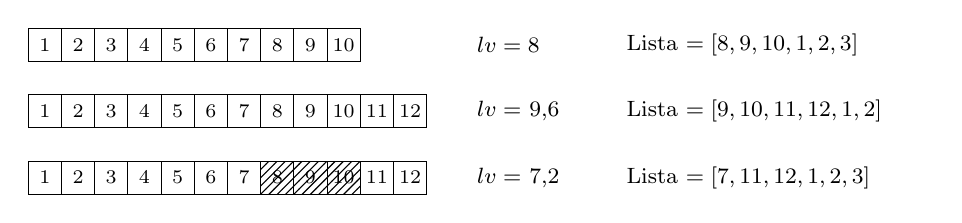
\begin{tikzpicture}[x=12pt, y=12pt]
        \tikzstyle{every node} = [font=\footnotesize]
        \tikzstyle{nu}  = [font=\scriptsize, draw, inner sep=0pt, minimum height=12pt, minimum width=12pt]
        \tikzstyle{st}  = [font=\scriptsize, draw, inner sep=0pt, minimum height=12pt, minimum width=12pt, pattern=north
                east lines]
        \tikzstyle{textul} = [node distance=1.6cm, inner sep=0pt, anchor=west, text width=2.6cm]
        \tikzstyle{stilcolb} = [inner sep=0pt, anchor=west, text width=1.4cm]
        \tikzstyle{stilcolc} = [inner sep=0pt, anchor=west, text width=3.9cm]

        \def\niva{0}
        \def\nivb{-2}
        \def\nivc{-4}
        \def\colb{14}
        \def\colc{18.5}

        \foreach[count=\c] \tip in {nu,nu,nu,nu,nu,nu,nu,nu,nu,nu}
            \node[\tip] at (\c,\niva) {\c};

        \foreach[count=\c] \tip in {nu,nu,nu,nu,nu,nu,nu,nu,nu,nu,nu,nu}
            \node[\tip] at (\c,\nivb) {\c};

        \foreach[count=\c] \tip in {nu,nu,nu,nu,nu,nu,nu,st,st,st,nu,nu}
            \node[\tip] at (\c,\nivc) {\c};

        \node[stilcolb] at (\colb,\niva) {$lv=8$};
        \node[stilcolb] at (\colb,\nivb) {$lv=$ 9,6};
        \node[stilcolb] at (\colb,\nivc) {$lv=$ 7,2};

        \node[stilcolc] at (\colc,\niva) {Lista $=[8, 9, 10, 1, 2, 3]$};
        \node[stilcolc] at (\colc,\nivb) {Lista $=[9, 10, 11, 12, 1, 2]$};
        \node[stilcolc] at (\colc,\nivc) {Lista $=[7, 11, 12, 1, 2, 3]$};
    \end{tikzpicture}

    \caption{Evoluția listei de alocare pentru un client cu $n=6$ și $l=$ 0,8. La primul pas discul este continuu, la
    al doilea se adaugă 2 blocuri și la al treilea se șterg 3.}
    \label{fig:lievol}
\end{figure}

\begin{figure}[p]
    \centering
    % Setez unitățile în pt ca să aliniez mai ușor nodurile.
    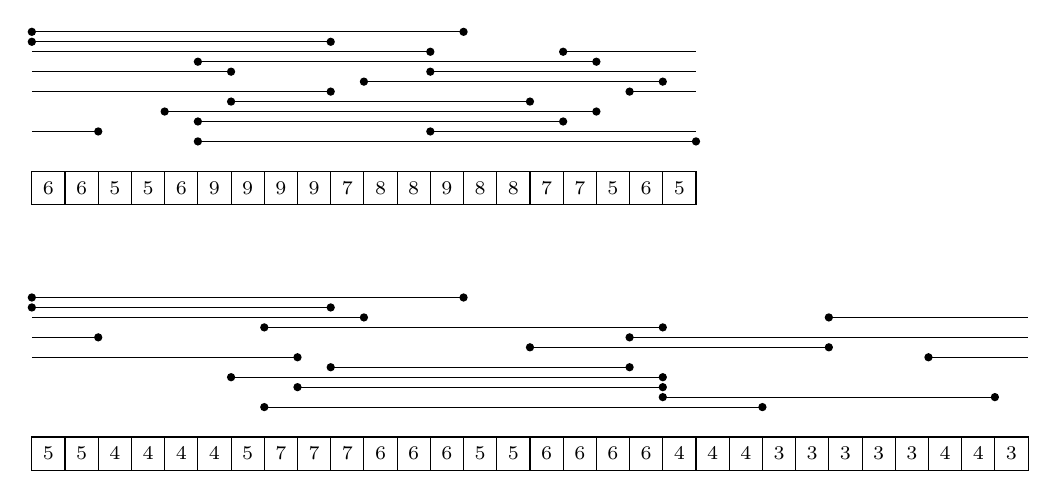
\begin{tikzpicture}[x=12pt, y=12pt]
        \tikzstyle{every node} = [font=\scriptsize]
        \tikzstyle{nu}  = [draw, inner sep=0pt, minimum height=12pt, minimum width=12pt]
        \tikzstyle{plin}  = [fill, circle, inner sep=0pt, minimum height=3pt, minimum width=3pt]
        \tikzstyle{textul} = [node distance=1.6cm, inner sep=0pt, anchor=west, text width=2.6cm]
        \tikzstyle{stilcolb} = [inner sep=0pt, anchor=west, text width=1.4cm]
        \tikzstyle{stilcolc} = [inner sep=0pt, anchor=west, text width=3.9cm]

        \def\depl{0.5}
        \def\sep{0.3}
        \def\va{20}

        \foreach[count=\c] \v in {6,6,5,5,6,9,9,9,9,7,8,8,9,8,8,7,7,5,6,5}
            \node[nu] at (\c,-5) {\v};
        \foreach[count=\c] \v in {5,5,4,4,4,4,5,7,7,7,6,6,6,5,5,6,6,6,6,4,4,4,3,3,3,3,3,4,4,3}
            \node[nu] at (\c,-13) {\v};

        \newcommand{\peers}[2]{
            \foreach[count=\c] \start/\enda/\endb in {#1} {
                \ifnum\endb>0
                    \draw (\depl+\start-1,-\c * \sep-#2) -- (\depl+\enda, -\c * \sep-#2);
                    \draw (\depl       , -\c * \sep-#2) -- (\depl+\endb, -\c * \sep-#2);
                    \node[plin] at (\depl+\start-1,-\c * \sep-#2){};
                    \node[plin] at (\depl+\endb,-\c * \sep-#2){};
                \else
                    \draw (\depl+\start-1, -\c * \sep-#2) -- (\depl+\enda, -\c * \sep-#2);
                    \node[plin] at (\depl+\start-1,-\c * \sep-#2){};
                    \node[plin] at (\depl+\enda,-\c * \sep-#2){};
                \fi
            }
        }

        \peers{1/13/0,1/9/0,17/20/12,6/17/0,13/20/6,11/19/0,19/20/9,7/15/0,5/17/0,6/16/0,13/20/2,6/20/0}{0}
        \peers{1/13/0,1/9/0,25/30/10,8/19/0,19/30/2,16/24/0,28/30/8,10/18/0,7/19/0,9/19/0,20/29/0,8/22/0}{8}
    \end{tikzpicture}

    \caption{Evoluția multiplicităților unui disc cu 20 de blocuri după adăugarea unui fișier cu 10 blocuri. Sunt 12
    parteneri în total și fiecare memorează între 8 și 15 blocuri.}
    \label{fig:limult}
\end{figure}

%%%%%%%%%%%%%%%%%%%%%%%%%%%%%%%%%%%%%%%%%%%%%%%%%%%%%%%%%%%%%%%%%%%%%%%%%%%%%%%%%%%%%%%%%%%%%%%%%%%%%%%%%%%%%%%%%%%%%%%%
\chapter*{Concluzii}
\addcontentsline{toc}{chapter}{Concluzii}

Am descris o soluție viabilă de menținere a unui sistem de fișiere continuu în rețea și cred că, dacă ar fi finisat, ar
putea înlocui folosirea serverelor BitTorrent private.

Există mai multe direcții de dezvoltare posibile. Sistemul poate fi îmbunătățit prin:

\begin{itemize}
    \item adăugarea unui sistem prin care clienții activi fac parte dintr-un flux prin care se pot publica eficient
    operațiile și intrarea noilor parteneri, astfel eliminându-se nevoia pentru un server pentru o rețea mică;
    \item adăugarea unui tabel distribuit de dispersie prin care să se facă comunicarea operațiilor și găsirea
    partenerilor;
    \item și adăugarea unei comunicări criptate.
\end{itemize}

%%%%%%%%%%%%%%%%%%%%%%%%%%%%%%%%%%%%%%%%%%%%%%%%%%%%%%%%%%%%%%%%%%%%%%%%%%%%%%%%%%%%%%%%%%%%%%%%%%%%%%%%%%%%%%%%%%%%%%%%
\begin{thebibliography}{99}
    \addcontentsline{toc}{chapter}{Bibliografie}
    \bibitem{proctf}
        \url{http://torrentfreak.com/bittorrent-still-king-of-p2p-traffic-090218/}
    \bibitem{wikitorr}
        \url{http://en.wikipedia.org/wiki/Torrent\_file}
    \bibitem{torrblk}
        \url{http://news.cnet.com/8301-13578\_3-9800629-38.html}
    \bibitem{dircon}
        \url{http://www.plop.nl/ptokaxbots/Mutor/DC-Protocol.htm}
    \bibitem{gnut1}
        \emph{The Gnutella Protocol Specification v0.4}
    \bibitem{gnut2}
        \url{http://en.wikipedia.org/wiki/Gnutella}
    \bibitem{freenet}
        I. Clarke, O. Sandberg, B. Wiley, T. W. Hong.
        \emph{Freenet: A Distributed Anonymous Information Storage and Retrieval System}
    \bibitem{wikifn}
        \url{http://en.wikipedia.org/wiki/Freenet}
    \bibitem{wikidfs}
        \url{http://en.wikipedia.org/wiki/Distributed\_file\_system}
    \bibitem{rfc1094}
        Sun Microsystems, Inc.
        \emph{NFS: Network File System Protocol Specification}\\
        \url{http://tools.ietf.org/html/rfc1094}
    \bibitem{wikip2ps}
        \url{http://en.wikipedia.org/wiki/List\_of\_file\_systems\#Peer-to-peer\_file\_systems}
    \bibitem{lucivy}
        A. Muthitacharoen, R. Morris, T. M. Gil, B. Chen.
        \emph{Ivy: A Read/Write Peer-to-Peer File System.}
        \emph{Proceedings of 5th Symposium on Operating Systems Design and Implementation}
        (OSDI 2002)
    \bibitem{lucpastis}
        J. M. Busca, F. Picconi, P. Sens.
        \emph{Pastis: a Highly-Scalable Multi-User Peer-to-Peer File System}
    \bibitem{luckadem}
        P. Maymounkov, D. Mazières.
        \emph{Kademlia: A Peer-to-peer Information System Based on the XOR Metric}
    \bibitem{testrez}
        \emph{Speed Comparison of Popular Crypto Algorithms}\\
        \url{http://www.cryptopp.com/benchmarks.html}
    \bibitem{md5broken}    
        \emph{Vulnerability Note VU\#836068: MD5 vulnerable to collision attacks} \\
        \url{http://www.kb.cert.org/vuls/id/836068}
    \bibitem{sha1crypt}
        \emph{Cryptanalysis of SHA-1} \\
        \url{http://www.schneier.com/blog/archives/2005/02/cryptanalysis\_o.html}
\end{thebibliography}

%%%%%%%%%%%%%%%%%%%%%%%%%%%%%%%%%%%%%%%%%%%%%%%%%%%%%%%%%%%%%%%%%%%%%%%%%%%%%%%%%%%%%%%%%%%%%%%%%%%%%%%%%%%%%%%%%%%%%%%%
\chapter*{Anexa 1}
\addcontentsline{toc}{chapter}{Anexa 1}

\begin{description}[style=multiline, leftmargin=5.0cm, font=\normalfont]
    \item[dosar:] director (în engleză \eng{directory} sau \eng{folder})
    \item[gestionar de dispunere:] \eng{layout manager} în engleză
    \item[mulțime de fire:] \eng{thread pool} în engleză
    \item[partener:] o instantă a unui program \eng{peer-to-peer}, care se manifestă ca un server (primind cereri și
    satisfăcându-le) și client (trimițând cereri) (în engleză \eng{peer})
    \item[rezumat:] funcție de rezumat sau funcție de dispersie (în engleză \eng{hash function})
    \item[roi:] la BitTorrent, mulțimea de parteneri (în engleză \eng{swarm})
    \item[\acr{TDD}:] tabel distribuit de dispersie (în engleză \eng{distributed hash table}, \acr{DHT})
    \item[șablon de proiectare:] \eng{design pattern} în engleză
    \item[torent:] toate fișierele care sunt descrise într-un fișier \cod{.torrent}
    \item[zona de notificare:] \eng{notification area} sau \eng{system tray} în engleză
\end{description}

\end{document}
